\documentclass[a4paper,12pt]{book}

% Paquetes necesarios
\usepackage[utf8]{inputenc}   % Codificación de caracteres
\usepackage[spanish]{babel}   % Idioma español
\usepackage[T1]{fontenc}      % Codificación de fuentes
\usepackage{amsmath, amssymb} % Símbolos matemáticos
\usepackage{graphicx}         % Inclusión de gráficos
\usepackage{cite}             % Gestión de citas
\usepackage{hyperref}         % Enlaces y referencias
\usepackage{geometry}         % Configuración de márgenes
\usepackage{fancyhdr}         % Encabezados y pies de página
\usepackage{titlesec}         % Formato de títulos
\usepackage{booktabs}         % Tablas profesionales
\usepackage{caption}          % Personalización de leyendas
\usepackage{enumitem}         % Personalización de listas
\usepackage{float}
\usepackage{tcolorbox}
\usepackage[table]{xcolor} % Paquete para colores en tablas
\usepackage{colortbl}       % Complemento para colorear celdas específicas
\usepackage{multirow}       % Combinar celdas en tablas
\usepackage{makecell}       % Combinar celdas en tablas
\usepackage{enumitem}
\usepackage{amsmath}
\usepackage{eurosym}
\usepackage{tikz}
\usepackage{listings}
\usepackage{color}
\usepackage{float}
\usepackage{pdfpages}

%\newcommand{\micode}[1]{\lstinline[basicstyle=\ttfamily, keywordstyle=\bfseries, breaklines=true]{#1}}      % Cargar el paquete listings

% Configuración para que listings soporte UTF-8
\lstset{
    extendedchars=true,  % Permite caracteres extendidos (opcional en versiones recientes)
    inputencoding=utf8,  % Asegura que listings entienda UTF-8
    breaklines=true,
    emphstyle=\itshape,
    basicstyle=\ttfamily, keywordstyle=\bfseries,
    literate={á}{{\'a}}1 {é}{{\'e}}1 {í}{{\'i}}1 {ó}{{\'o}}1 {ú}{{\'u}}1 
             {Á}{{\'A}}1 {É}{{\'E}}1 {Í}{{\'I}}1 {Ó}{{\'O}}1 {Ú}{{\'U}}1
             {ñ}{{\~n}}1 {Ñ}{{\~N}}1 {¿}{{¿}}1 {¡}{{¡}}1
}

% Definir \micode con soporte para tildes
\newcommand{\micode}[1]{\lstinline{#1}}

%creacion de un lstlisting claro y bonito
\lstdefinestyle{mystyle}{
    backgroundcolor=\color{white},   
    commentstyle=\color{green},
    keywordstyle=\color{blue},
    numberstyle=\tiny\color{gray},
    stringstyle=\color{red},
    basicstyle=\ttfamily\footnotesize,
    breakatwhitespace=false,         
    breaklines=true,                 
    captionpos=b,                    
    keepspaces=true,                 
    numbers=left,                    
    numbersep=5pt,                  
    showspaces=false,                
    showstringspaces=false,
    showtabs=false,                  
    tabsize=2
}

\lstdefinestyle{yamlstyle}{
    backgroundcolor=\color{yellow!10},   
    commentstyle=\color{purple},
    keywordstyle=\color{orange},
    numberstyle=\tiny\color{blue},
    stringstyle=\color{teal},
    basicstyle=\ttfamily\footnotesize\bfseries,
    breakatwhitespace=false,         
    breaklines=true,                 
    captionpos=b,                    
    keepspaces=true,                 
    numbers=left,                    
    numbersep=5pt,                  
    showspaces=false,                
    showstringspaces=false,
    showtabs=false,                  
    tabsize=2,
    morekeywords={true,false,null,y,n}
}

\lstdefinestyle{directorystructure}{
    backgroundcolor=\color{gray!10},   
    commentstyle=\color{green!50!black},
    keywordstyle=\color{blue!70},
    numberstyle=\tiny\color{gray},
    stringstyle=\color{red!70!black},
    basicstyle=\ttfamily\footnotesize,
    breakatwhitespace=false,         
    breaklines=true,                 
    captionpos=b,                    
    keepspaces=true,                 
    numbers=none,                    
    showspaces=false,                
    showstringspaces=false,
    showtabs=false,                  
    tabsize=2
}

\lstnewenvironment{directorylisting}[1][]{
    \lstset{
        style=directorystructure,
        caption={#1},
        frame=single,
        framerule=0.5pt,
        rulecolor=\color{black!50},
        xleftmargin=0.5cm,
        xrightmargin=0.5cm
    }
}{}



\setlength{\headheight}{14.5pt}

% Configuración de márgenes
\geometry{left=3cm, right=3cm, top=2.5cm, bottom=2.5cm}

% Configuración de encabezados y pies de página
% \setlength{\headheight}{14.49998pt}
\pagestyle{fancy}
\fancyhf{}
\fancyhead[L]{Universidad de Granada}
\fancyhead[L]{\nouppercase{\leftmark}}

% \fancyhead[C]{Escuela Técnica Superior de Ingenierías Informática}
\fancyhead[R]{Ingeniería de Servidores}
\fancyfoot[L]{\rule[0pt]{\textwidth}{0.2pt}\\Ismael Sallami Moreno}
\fancyfoot[C]{\rule[0pt]{\textwidth}{0.2pt}\\\thepage}
\fancyfoot[R]{\rule[0pt]{\textwidth}{0.2pt}\\\today}
\renewcommand{\sectionmark}[1]{\markboth{#1}{}} % Configura \leftmark para que solo muestre la sección


% Formato de títulos
\titleformat{\section}{\large\bfseries}{\thesection.}{0.5em}{}
\titleformat{\subsection}{\normalsize\bfseries}{\thesubsection.}{0.5em}{}

% Datos del documento
\title{\textbf{Prácticas Ingeniería de Servidores}}
\author{
    Ismael Sallami Moreno \\
    \texttt{ism350zsallami@correo.ugr.es}
}
\date{
    \vspace{1cm}
    \begin{tabular}{rl}
        \textbf{Asignatura:} & Ingeniería de Servidores \\
        \textbf{Tema:} & Prácticas \\
        \textbf{Fecha:} & \today
    \end{tabular}
}

\begin{document}

% Portada
\begin{titlepage}
    \begin{center}
        % \vspace*{1cm}
        
        % \Huge
        % \textbf{Práctica Contabilidad Financiera II}
        \Huge \textbf{Prácticas Ingeniería de Servidores} 
        % \vspace{0.5cm}
        % \LARGE
        % \textbf{Ismael Sallami Moreno}\\
        % \LARGE
        % \texttt{ism350zsallami@correo.ugr.es}
        % \LARGE
        % \url{https://github.com/Ismael-Sallami}
        
        % \vfill
        
        % \Large
        % \textbf{Universidad de Granada}
        
        \vspace{0.8cm}
        
        \begin{tikzpicture}[remember picture, overlay]
            \node[opacity=0.2] at (current page.center) {
\includegraphics[width=\paperwidth,height=\paperheight]{portada.jpg}};
            \node[align=center] at (current page.center) {
                
                \vspace{0.5cm}
                \LARGE \textbf{Ismael Sallami Moreno} \\
                \LARGE \texttt{ism350zsallami@correo.ugr.es} \\
                \LARGE \url{https://ismael-sallami.github.io/} \\
                \LARGE \url{https://elblogdeismael.github.io/} \\
                \vspace{2cm}
                \Large \textbf{Universidad de Granada} \\
                \vspace{0.8cm}
                % \Large \textbf{2025}
            };
        \end{tikzpicture}
        \vfill
        
        \Large
        \textbf{2025}
        
    \end{center}
\end{titlepage}
\newpage


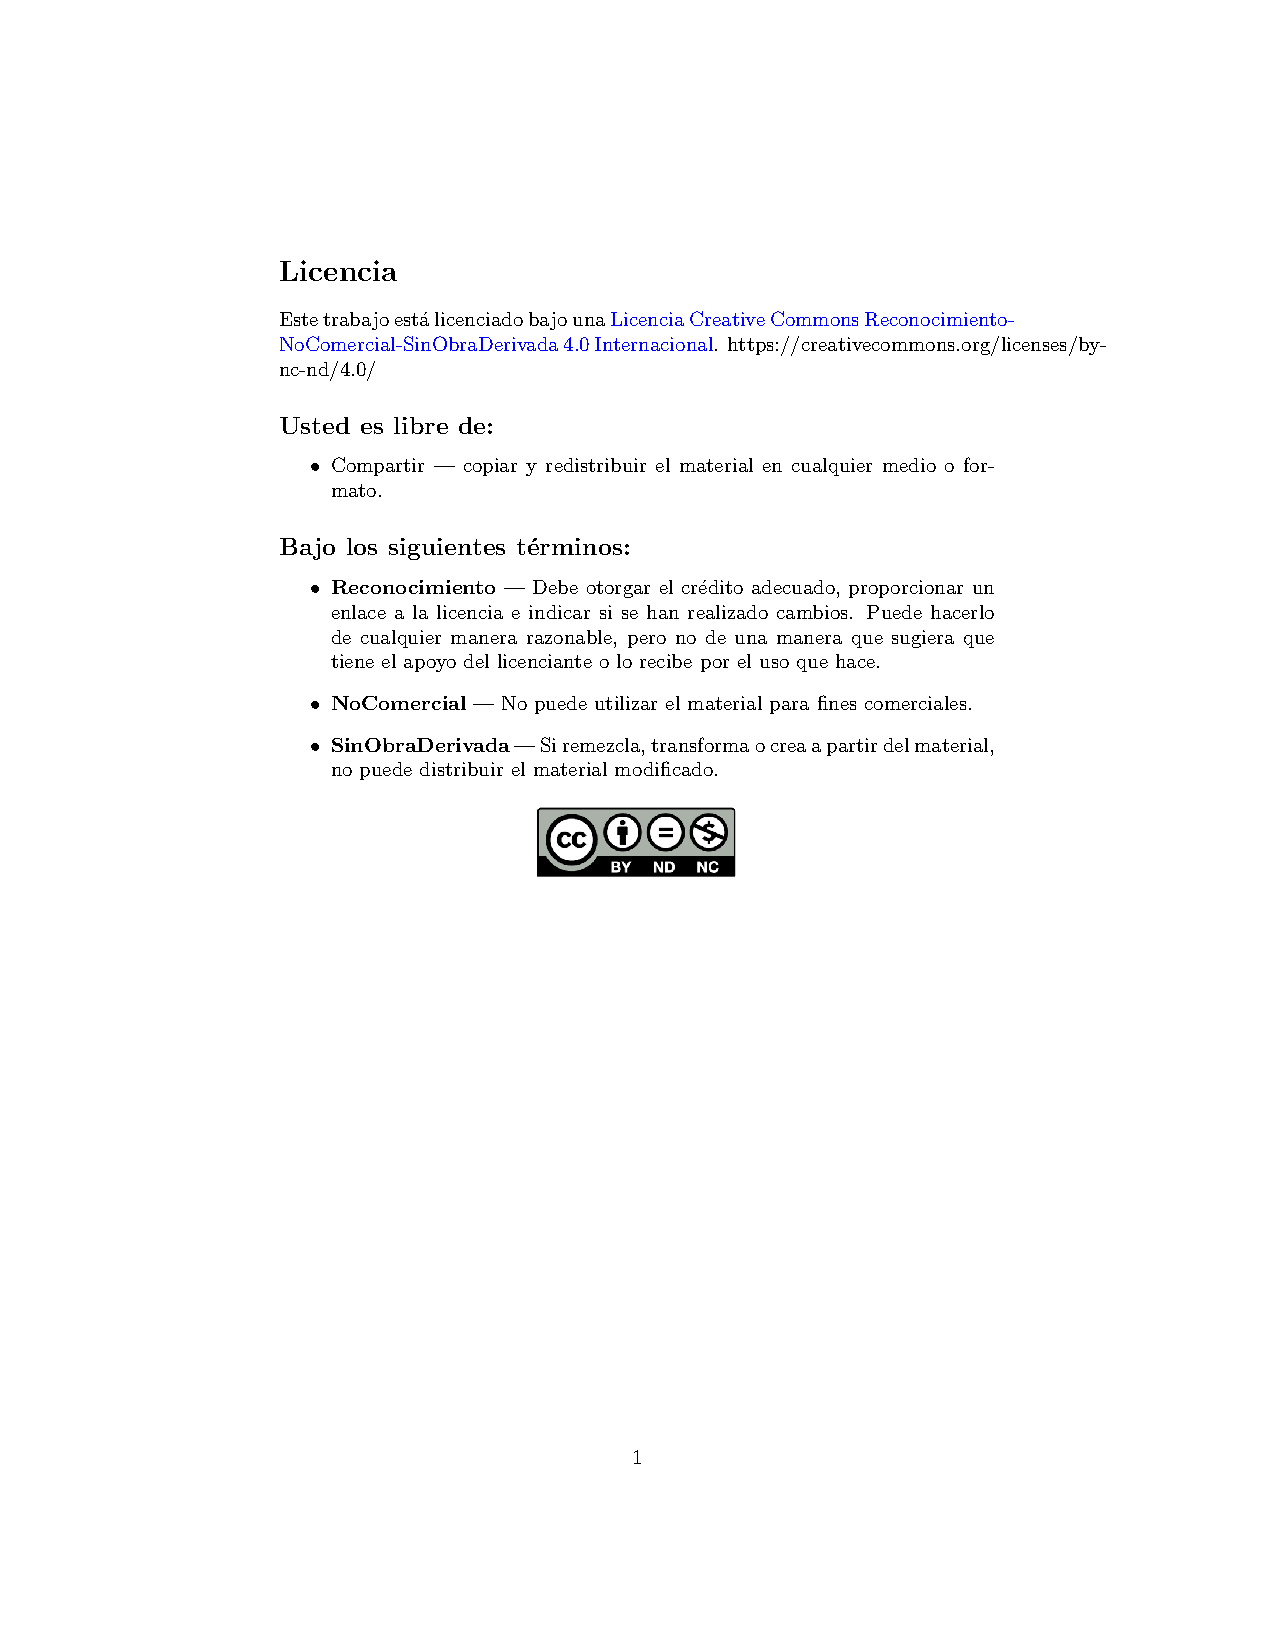
\includepdf[pages=-]{../../../../../licencia.pdf}
% Tabla de contenidos
\tableofcontents
\newpage

\part{Apuntes de Clase}

\chapter{Bloque 1}

\section{Ping y SSH}

Sobre esta parte no decidí tomar apuntes en clase debido a que son conceptos vistos en la Asignatura de Fundamentos de Redes, por lo que consideré que no era necesario. De todas formas en la parte de Prácticas (Resolución) se comenta paso a paso lo que se hizo en esta parte.
\newpage
\section{LVM y RAID}

\subsection{LVM (Logical Volume Manager)}

\begin{itemize}
    \item \textbf{Discos y particiones}:
    \begin{itemize}
        \item \micode{sda}: Primer disco del sistema.
        \item Luego pueden existir \micode{sdb}, \micode{sdc}, etc.
    \end{itemize}
    \item Consideraciones importantes:
    \begin{itemize}
        \item Si el directorio \micode{/boot} se llena, el sistema podría fallar al arrancar debido a la falta de espacio disponible.
        \item Se recomienda evitar el uso de \micode{swap} en sistemas virtualizados, ya que reduce el rendimiento.
    \end{itemize}
\end{itemize}

\subsection{Directorios base en Linux}
\begin{itemize}
    \item \textbf{/boot}: Contiene los archivos de arranque del sistema.
    \item \textbf{/etc}: Almacena los archivos de configuración del sistema operativo.
    \item \textbf{/dev}: Contiene archivos especiales que representan dispositivos del sistema.
    \item \textbf{/mnt}: Punto de montaje temporal para sistemas de archivos.
    \item \textbf{/var}: Contiene datos variables del sistema, como logs y archivos temporales. Puede crecer mucho, por lo que se recomienda monitorearlo.
\end{itemize}

\subsection{RAID (Redundant Array of Independent Disks)}

RAID es una tecnología que permite combinar múltiples discos para mejorar la redundancia y/o el rendimiento del sistema de almacenamiento.

\subsection{Ventajas}
\begin{itemize}
    \item Permite unir volúmenes de almacenamiento.
    \item Mejora el rendimiento si los discos están en buses distintos, ya que permite acceso en paralelo.
\end{itemize}

\subsection{Niveles de RAID}
\begin{itemize}
    \item \textbf{RAID 0 (Striping)}:
    \begin{itemize}
        \item Divide los datos en bloques y los distribuye entre varios discos.
        \item \textbf{Problema}: Si un disco falla, se pierde toda la información.
        \item Se usa poco en la práctica debido a su baja robustez.
    \end{itemize}
    
    \item \textbf{RAID 1 (Mirroring)}:
    \begin{itemize}
        \item Duplica los datos en dos o más discos.
        \item Si un disco falla, el otro sigue funcionando con los mismos datos.
        \item Aporta robustez al sistema.
        \item \textbf{Problema}: Se paga el doble en almacenamiento.
        \item Se usa frecuentemente en \micode{/boot} para garantizar que el sistema pueda arrancar en caso de fallo de un disco.
    \end{itemize}
    
    \item \textbf{RAID 5 (Paridad distribuida)}:
    \begin{itemize}
        \item Se distribuyen los datos y la paridad entre todos los discos.
        \item Si un disco falla, se pueden recuperar los datos utilizando la paridad.
        \item \textbf{Problema}: Puede reducir el rendimiento debido al tiempo necesario para calcular la paridad.
        \item \textbf{Ventaja}: Equilibra costos, robustez y capacidad de recuperación.
        \item Se puede usar un disco de repuesto que entra en acción si uno falla.
    \end{itemize}
\end{itemize}

\subsection{Tipos de RAID}
\begin{itemize}
    \item \textbf{RAID por Hardware}: 
    \begin{itemize}
        \item Utiliza un controlador RAID físico.
        \item Es más eficiente y transparente para el sistema operativo.
    \end{itemize}
    
    \item \textbf{RAID por Software}: 
    \begin{itemize}
        \item Administrado por el sistema operativo.
        \item Puede ser modificado por el administrador, lo que representa un riesgo.
        \item Requiere más recursos del sistema.
    \end{itemize}
\end{itemize}

\subsection{Ejercicio Opcional: Configuración de RAID1 para /var}

\subsection{Objetivo}
El objetivo es proporcionar a \micode{/var} un respaldo frente a fallos mediante la creación de un RAID1. Para ello, debemos montar un RAID1 y mover \micode{/var} dentro de este.

\subsection{Pasos a seguir}
\begin{enumerate}
    \item \textbf{Creación de discos virtuales en la máquina virtual (MV)}
    \begin{itemize}
        \item Se crean dos discos: \micode{raid1} y \micode{raid2}.
        \item Usamos \micode{lsblk} para verificar la existencia de \micode{sdb} y \micode{sdc}.
    \end{itemize}

    \item \textbf{Instalación de \micode{mdadm}}
    \begin{itemize}
        \item \micode{sudo dnf provides mdadm} (para verificar qué paquete lo proporciona).
        \item \micode{sudo dnf install mdadm} (para instalarlo).
    \end{itemize}

    \item \textbf{Creación del RAID1}
    \begin{itemize}
        \item \micode{sudo mdadm --create /dev/md0 --level=1 --raid-devices=2 /dev/sdb /dev/sdc}
        \item Aparecerá un \textit{warning} sobre la creación de metadatos, confirmamos con "sí".
        \item Para monitorear la sincronización del RAID:  
              \micode{watch -n 1 more /proc/mdstat}
        \item Luego, verificamos con \micode{lsblk}.
    \end{itemize}

    \item \textbf{Prueba de fallo de disco}
    \begin{itemize}
        \item Podemos simular la falla de un disco con:  
              \micode{echo 1 > /dev/sdb}
        \item Se observa que \micode{md0} sigue funcionando al ser un \textit{mirror}.
    \end{itemize}
\end{enumerate}

\subsection{LVM (Logical Volume Manager)}

\subsection{Conceptos Clave}
\begin{itemize}
    \item \textbf{LV (Logical Volume)}
    \item \textbf{VG (Volume Group)}
    \item \textbf{PV (Physical Volume)}
\end{itemize}

La estructura básica de LVM es la siguiente:

\begin{verbatim}
    LV         LV   
    '           '
   Volumen Group  
       '
   '     '     '
  pv    pv    pv  
\end{verbatim}

Un \textbf{Logical Volume (LV)} puede expandirse tomando espacio libre de otros discos o estructuras.

\subsection{Visualización de LVM}
\begin{itemize}
    \item Para ver los discos que son de tipo LVM, usamos \micode{lsblk} en la columna de \textit{type}.
    \item Para ver opciones de \micode{pv}, \micode{vg} y \micode{lv}, usamos \micode{tab-completion}.
\end{itemize}

\subsection{Consideraciones sobre Volumen Groups}
Si un \textbf{Volume Group} contiene un disco magnético, un SSD y un RAID, el acceso a los datos puede no ser homogéneo. Por ello, el volumen lógico debe montarse sobre el RAID.

\subsection{Creación del LVM sobre el RAID}
\begin{enumerate}
    \item Convertir el RAID en un Physical Volume:
          \micode{pvcreate /dev/md0}
    \item Crear un Volume Group llamado \micode{raid1}:
          \micode{vgcreate raid1 /dev/md0}
    \item Crear un Logical Volume de 10GB dentro del Volume Group:
          \micode{lvcreate -L 10G -n rvar raid1}
\end{enumerate}

\subsection{Movimiento de /var al RAID}
Después de crear el volumen lógico, debemos mover \micode{/var} dentro del RAID:

\begin{itemize}
    \item El nombre del volumen dentro del RAID es \micode{/dev/raid1/rvar}.
    \item También puede aparecer como \micode{/dev/mapper/raid1-rvar}, ya que son sinónimos creados mediante enlaces simbólicos.
\end{itemize}

\subsection{Resolución de Problemas}

\subsection{Problema 1: Configurar el sistema de archivos en \micode{rvar}}

Actualmente, el volumen lógico \micode{rvar} está vacío y sin un sistema de archivos. Para solucionarlo, seguimos estos pasos:

\begin{enumerate}
    \item \textbf{Seleccionar un sistema de archivos:}  
    Los sistemas de archivos recomendados son \textbf{ext4} y \textbf{xfs}, ya que son transaccionales y previenen la corrupción de datos en caso de fallos.  
    \item \textbf{Verificar los sistemas de archivos soportados:}  
    Ejecutamos el siguiente comando para listar los sistemas disponibles en el kernel:
    \begin{verbatim}
    ls /lib/modules/$(uname -r)/kernel/fs
    \end{verbatim}
    \item \textbf{Formatear el volumen lógico con \micode{ext4}:}
    \begin{verbatim}
    mkfs.ext4 /dev/mapper/raid1-rvar
    \end{verbatim}
\end{enumerate}

\subsection{Problema 2: Montar y trasladar /var al nuevo volumen}

El volumen lógico \micode{rvar} debe ser montado en el sistema y debemos trasladar \micode{/var} sin perder datos. Para ello:

\begin{enumerate}
    \item \textbf{Montar el volumen lógico:}  
    Primero, montamos \micode{rvar} en un directorio temporal:
    \begin{verbatim}
    mount /dev/mapper/raid1-rvar /mnt/
    \end{verbatim}
    Podemos verificar con:
    \begin{verbatim}
    mount
    \end{verbatim}
    Al revisar \micode{/mnt/}, aparecerá el directorio \micode{lost+found}, indicando que el sistema de archivos está activo.

    \item \textbf{Cambiar a modo mantenimiento:}  
    Para evitar la pérdida de datos al copiar \micode{/var}, debemos entrar en el \textbf{runlevel1}, también conocido como \textbf{modo mantenimiento}. Esto se hace con:
    \begin{verbatim}
    systemctl isolate runlevel1.target
    \end{verbatim}
    Podemos confirmar el estado con:
    \begin{verbatim}
    systemctl status
    \end{verbatim}

    \item \textbf{Copiar los datos de /var a /mnt/}:  
    Copiamos todo el contenido de \micode{/var} manteniendo atributos con:
    \begin{verbatim}
    cp -a /var/* /mnt/
    \end{verbatim}

    \item \textbf{Crear un respaldo de /var:}  
    Antes de reemplazar \micode{/var}, hacemos una copia de seguridad por si algo falla:
    \begin{verbatim}
    mv /var /var_old
    \end{verbatim}

    \item \textbf{Desmontar /mnt y montar el nuevo /var:}  
    \begin{verbatim}
    umount /mnt
    mkdir /var
    mount /dev/mapper/raid1-rvar /var
    \end{verbatim}
    Podemos verificar con:
    \begin{verbatim}
    df -h
    \end{verbatim}

    \item \textbf{Hacer el montaje permanente en \micode{/etc/fstab}:}  
    Si reiniciamos ahora, la configuración se perdería. Para evitarlo, editamos el archivo \micode{/etc/fstab} y agregamos la siguiente línea:
    \begin{verbatim}
    /dev/mapper/raid1-rvar      /var       ext4     defaults     0 0
    \end{verbatim}
    
    \item \textbf{Probar la configuración antes de reiniciar:}  
    \begin{verbatim}
    mount -a
    systemctl daemon-reload
    mount
    \end{verbatim}
    Si todo está correcto, reiniciamos el sistema.
\end{enumerate}

\subsection{Interpretación de \micode{lsblk}}

El comando \micode{lsblk} nos permite visualizar la estructura de almacenamiento del sistema. Es importante identificar:

\begin{itemize}
    \item \textbf{Discos físicos y particiones}: Aparecen como \micode{sda}, \micode{sdb}, \micode{sdc}, etc.
    \item \textbf{Volúmenes lógicos}: Se muestran bajo \micode{/dev/mapper/}.
    \item \textbf{SR0}: Indica la unidad de CD-ROM.
\end{itemize}

\newpage
\section{Firewall + SSHD}

Ya sabemos de otras Asignaturas que un \textbf{firewall} es un sistema que controla el tráfico de red, permitiendo o bloqueando ciertas conexiones. En Linux, el firewall más común es \textbf{iptables}.

El comando que tenemos que aprender a gestionar es \micode{firewall-cmd}, tiene diversas opciones como status, state. Otra forma para ver si esta arrancado es \micode{systemctl status firewall}.

Otras opciones: \micode{firewall-cmd --list-all}, en este comando debemos de ver los filtros que estan definidos, en services podemos ver los servicios que están habilitados.

Con sudo firewall-cmd --add-service=http, cuando lo listo otra vez, se añade el puerto http en la opción services. Cuando se hace con firewall-cmd, se hace dinámica, por lo que si reiniciamos esto se pierde. Para que se quede debemos de ejecutar el comando \micode{sudo fire firewall-cmd --runtime-to-permanent}. De forma alternativa, podemos ejecuar primero la opción \micode{--permanent} y luego \micode{--add-port=443/http}, pero si lo listamos no lo lleva a memoria, no hay ninguna opción que lo deje permanente y que lo lleve a memoria. Tenemos dos opciones o trabajar con servicios o llevarlo a memoria.

Si queremos conocer los servicios, podemos ejecutar \micode{firewall-cmd --get-services}.

Los firewalls en Linux son muy eficientes debido a que en este SO se trabaja con servicios, por lo que se puede controlar el tráfico de forma muy precisa. Al implementarse a nivel de Kernel ayuda a que sea muy eficiente.
\textit{No se va a preguntar nada sobre iptables}.

Debemos de usar el programa \micode{nmap} ya que nos dice que puertos están abietos en un servidor. Para instalarlo, usamos \micode{sudo dnf install nmap}. En el guión debemos de mirar la referenia número 31.

\subsection{Ejercicio Opcional}

Debemos de instalar un servicio HTTP, se recomienda Apache. Podemos escanear los 100 puertos mas usados con el comando \micode{nmap -F localhost}. Para instalar Apache, usamos \micode{sudo dnf install httpd}. Para arrancar el servicio, usamos \micode{sudo systemctl start httpd}. Para comprobar que está arrancado, usamos \micode{sudo systemctl status httpd}. Para que arranque en el inicio, usamos \micode{sudo systemctl enable httpd}. Para comprobar que está escuchando en el puerto 80, usamos \micode{sudo ss -tulnp | grep 80}.

Debemos de poder acceder desde el navegador de la máquina anfitrión.

\subsection{SSH}

Es un programa de terminal remoto, ya lo hemos usado en Asignaturas anteriormente. Antes se usaba Telnet, en este se especifica la dirección IP y el puerto, pero no era seguro, por lo que cualquier man in the middle podía interceptarlo y suplantar la identidad. Además, todas las respuestas que se producían eran en abierto, los \micode{cat},... En cambio, SSH es seguro, ya que se cifra la información. Este hace lo mismo que Telnet, pero de forma segura. Se recomienda hacerlo \micode{ssh usuario@ip}. O bien sustituir la IP por el nombre del dominio. Para cerrar la conexión, usamos \micode{exit}. 

Ya hemos estudiado en otras Asignaturas el tema de criptografía en cuanto al cifrado simétrico y asimétrico. En especial, en Fundamentos de Redes. Por si acaso, vamos a hacer una pequeña introducción. Tenemos dos tipos de cifrado:
\begin{itemize}
    \item \textbf{Cifrado simétrico}: Se usa una clave para cifrar y descifrar. El problema es que si alguien intercepta la clave, puede descifrar todo. Por ello, se usa poco.
    \item \textbf{Cifrado asimétrico}: Se usa una clave pública para cifrar y una privada para descifrar. La clave pública se puede compartir, pero la privada no. Se usa para firmar documentos, ya que si se cifra con la clave privada, solo se puede descifrar con la clave pública.
\end{itemize}

Debemos de destacar los conceptos de \textbf{autenticación} y \textbf{autorización}. La autenticación es el proceso de verificar la identidad de un usuario, mientras que la autorización es el proceso de verificar si un usuario tiene permiso para acceder a un recurso. Además, del uso de certificados digitales, que son un tipo de credencial que se usa para autenticar la identidad de un usuario o un servidor. Este se consigue a través de una entidad certificadora, usando una clave pública y privada (Big Brother).

Algoritmos :
\begin{itemize}
    \item Llave simétrica: DES(tenemos dos llaves, una que es privada y otra que es pública, lo que se cifra con la privada solo se puede descifrar con la pública, por dentro se gestiona en base a números primos muy grandes).
    \item Llave asimétrica: RSA (Se guarda la privada, mientras que la pública se comparte, estando incluso compartida en la propia web, de manera que la persona que quiera compartir contigo usa la pública para codificar el texto y te lo manda codificado, de esta manera si hay un man in the middle lo ve cifrado, solo la persona con la llave privada puede ver su contenido).
\end{itemize}

Otro uso de la llave privada es la \textit{firma}, de esta manera se garantiza la confidencialidad y la autenticación del mensaje debido a que es confidencial debido a que solo se puede descifrar con la llave pública, y autenticidad debido a que solo se puede cifrar con la llave privada, la cual solo conoce esa entidad.

Firma Digital: Usando Hash SHA256, se cifra con la llave privada y se envía el mensaje cifrado y el mensaje en abierto. La persona que recibe el mensaje cifrado con la llave privada, lo descifra y lo compara con el mensaje en abierto, si son iguales, se garantiza la autenticidad del mensaje. Ejemplo de ello puede ser el minado de monedas como es el Bitcoin. Además, otro ejemplo de ello es cuando descargamos algo y podemos verificar que es el del propio distribuidor usando el Hash que me proporciona. \textit{Por ende, podemos cosiderar que un HASH + llave privada es el certificado digital}. Para asegurarnos de que la llave pública es de quien dice ser debemos de ver el certificado digital, como hemos mencionado anteriormente. Este proceso para cuando encontramos un certificado digital que es de confianza, ya que si no lo es, no podemos asegurar que la llave pública sea de quien dice ser. Para ver los certificados, vemos que en Firefox, accedemos a settings y buscamos \textit{certificados}, podemos ver las entidades que nuestro browser reconoce.

\begin{tcolorbox}[colback=yellow!10!white, colframe=red!75!black, title=Advertencia]
El tema de certificados y demás al ser materia de Fundamentos de Redes, no se va a preguntar en el examen.
\end{tcolorbox}

Nos conectamos a un ordenador remoto mediante ssh, de esta manera le decimos que nos queremos conectar, el te envía la llave pública, es decir, se va a su configuración, recupera la llave y te la envía. A continuación, le enviamos nuestras creedenciales cifradas con la llave pública, y cuando le llega, las descifra con la llave privada y comprueba si son correctas. Si lo son, nos deja entrar. Si no lo son, nos dice que no podemos entrar. Además, de esta manera se prevee que un \textit{man-in-the-middle} no pueda interceptar las credenciales.

Podemos meterle una entrada en el fichero de host, de esta manera cuando nos conectamos a un servidor, nos conectamos a una IP, pero si le metemos una entrada en el fichero de host, le decimos que esa IP es un nombre, de esta manera cuando nos conectamos a ese nombre, nos conectamos a esa IP. Para ello, debemos de editar el fichero \micode{/etc/hosts} y añadir la IP y el nombre del servidor, así es más cómdo, para ello en Linux es \micode{ssh usuario@nombre}. 

Cuando ejecutamos el comando para conectarnos, nos imprime un mensaje con el HASH, y nos pregunta que si nos lo creemos, si en vez de una llave pública esta reconocida en nuestras llaves y ve que tenemos el certificado no nos preguntaría. En todos lo equipos se crea el directorio ssh en home, dentro de este tenemos un archivo que se llama known\_hosts, el cual contiene las llaves públicas de los ordenadores que ya has confiado, de manera que no nos va a preguntar cuando nos conectemos de nuevo, si queremos que en la primera vez tampoco pregunta la copiamos y pegamos, entre otras opciones. \textit{Nota: Por defecto se crea ese directorio cuando se conetca por ssh.}

Este proceso es muy costos en términos de cómputo, por lo que se usa lo más mínimo posible. Por esto se usa un proceso de handshaking, de esta manera el equipo le manda una propuesta de llave simétrica y de esta manera ya se usa en adelante, ya que el uso de clave privada y pública es muy costoso.

¿Cómo puedo acceder sin contraseña? Para ello nos autenticamos con llave pública y llave privada. En el caso de que decidamos hacerlo asi cuando le mandamos que soy 'nombre', recupera la llave de el directorio .ssh y le manda un mensaje de firmame esto con la clave privada de dicho usuario, y de esta manera se asegura de que efectivamente es el usuario que dice ser. Además, en el directorio home solo puede escribir el usuario y el root.

En la MV:

\begin{itemize}
    \item ssh-keygen: crea la llave privada dentro de home, luego nos pregunta si queremos protegerla con contraseña, si no queremos, le damos a enter, \textit{pero siempre debe de hacerse.} Luego si nos vamos al directorio vemos dos documentos la llave privada y la pública. Si queremos que no nos pregunte siempre la contraseña, usamos el comando \micode{ssh-agent}, de esta manera el la escribe por ti, hasta que usamos el comando \micode{exit}, en este caso se olvida.
\end{itemize}

Para usar la pública:
\begin{itemize}
    \item Accedemos al directorio /home/.ssh 
    \item usamos el comando ssh-copy-id usuario@{ip/hostname} (copia mi identidad, se puede hacer con ctrl+c/v), y luego nos hace una prueba para que le demostremos que de verdad somos el usuario al que nos queremos conectar, para ello le mandamos la contraseña.
    \item Luego comprobamos que podemos entrar sin contraseña.
    \item En la máquina donde nos hemos conectado, vemos un fichero llamado \textit{id\_rsa.pub}, y si lo listamos debe de ser el mismo que la clave pública de la máquina inicial, desde la que nos conectamos a esta.
\end{itemize}

\textit{Nota: El directorio .ssh se crea en el home cuando es el cliente, mientras que en el servidor se crea en el /etc/ssh, también podemos crearlo nosotros a priori.}

Ahora podemos ejecuar un comando remoto, por ejemplo: \micode{ssh usuario@ip comando}, de esta manera se ejecuta el comando en la máquina remota. En este punto comienza la automatización de configuración remota. \textit{Ansible son scripts pero ejecutados de manera remota.} Además, podemos copiar archivos usando el comando scp (secure copy), de esta manera se copia el archivo de una máquina a otra. \textit{Nota: scp es un comando de ssh.} El comando es \micode{scp origen destino}, por ejemplo: \micode{scp /home/usuario/archivo usuario@ip:/home/usuario/}, de esta manera se copia el archivo de la máquina local a la remota. Si queremos copiar un directorio, usamos el comando \micode{scp -r origen destino}. Además podemos conectarnos mediante \textit{sftp} (secure file transfer protocol), de esta manera se conecta a la máquina remota y podemos copiar archivos de manera interactiva. \textit{Nota: sftp es un comando de ssh.} Para conectarnos, usamos el comando \micode{sftp usuario@ip}, y luego podemos usar los comandos \micode{put} y \micode{get} para copiar archivos de una máquina a otra.

\subsection{Ejercicio Opcional}

En el ejercicio debemos de dar acceso mediante ssh usando la llave pública y privada, debemos de modificar el puerto para conectarnos en vez del 22 para el ssh usar otro que sea mayor que el 1024, para ello podemos asegurarnos de que no estamos colisionando con un puerto conocido buscando en Innternet.

\begin{enumerate}
    \item Accedemos al contenido del demonio del ssh que se encuentra en /etc/ssh, una vez dentro nos pone el comando que debemos de ejecuar \micode{semanage...} (aparece en el fichero de ssh de la máquina Rocky), para que se apliquen los cambios debemos de reiniciar el servicio, para ello usamos el comando \micode{sudo systemctl restart sshd} o bien reiniciar la máquina.
    \item Además debemos de modificar el firewall para permitir ese puerto, para ello usamos el comando \micode{sudo firewall-cmd --add-port=puerto/tcp --permanent}, y luego reiniciamos el servicio con \micode{sudo systemctl restart firewalld}.
    \item Luego debemos de copiar la llave pública a la máquina remota, para ello usamos el comando \micode{ssh-copy-id usuario@ip}, y luego nos pide la contraseña, una vez introducida, ya podemos conectarnos sin contraseña.
    \item Para comprobar que todo está correcto, usamos el comando \micode{ssh usuario@ip -p puerto}, de esta manera nos conectamos a la máquina remota.
\end{enumerate}

Con el parámetro -p le especificamos el puerto al que nos queremos conectar, de esta manera nos conectamos al puerto que hemos especificado, ya que de manera predeterminada se conecta al puerto 22.

\section{Automatización con Ansible}

Por defecto Ansible ya viene instalado en la mayoría de las distribuciones de Linux. Además, por defecto al instalar Ansible se instala Python y SSH. Para instalarlo debemos de usar el comando \micode{sudo dnf install ansible}. Para comprobar que está instalado, usamos el comando \micode{ansible --version}, o bien mediante el comando \micode{sudo dnf list installed | grep -i ansible}. Además, podemos ver la documentación de Ansible en la página oficial de Ansible. Su configuración se encuentra en /etc/ansible, \textit{este solo se instala en el controlador ya que es desde donde se maneja.}

En la configuración de /etc/ansible, podemos cambiar varios parámetro, como es el caso del número de hebras que usa o número de procesos que se ejecutan de manera pararela, en este caso suele estar por defecto en 5 hebras.

En nuestro directorio base\footnote{Accedemos con el comando \micode{cd}.}, tenemos el archivo \micode{.ansible.cfg}, el cual podemos editar siendo los cambios aplicados de la misma manera que si lo hiciéramos en el archivo de configuración de /etc/ansible. Por defecto viene vacío, pero tiene un comando para generar la configuración por defecto, el cual es \micode{ansible-config dump}. Además, podemos ver la configuración de Ansible con el comando \micode{ansible-config list}.

En cuanto al formato que se usa en Ansible, cabe destacar que se establecen etiquetas, como puede ser \micode{web server}, de manera que cuando ejecutemos Ansible, podemos elegir esta etiqueta para que lo lance con lo que esté definido debajo de dicha etiqueta en el archivo de configuración.

Entramos en ansible con \micode{cd .ansible}, y debemos de definir etiquetas para entrar a los hosts que se definen en este archivo de configuración. En este archivo se definen los hosts. 

Una de las referencias importante es la guía sobre AD-HOC y la lista de todos los módulos que podemos ejecutar\footnote{Referencias 42 y 43 del guión.}. LOs módulos que vienen po defecto son los \textit{ansible.builtin}. El pinf de Ansible, actúa de manera distinta, lo que hace es que comprueba si se tiene acceso al servidor al que se hace el ping y comprueba si este tiene pyhton instalado. Solo se le pasa un parámetro.

Para ejecutar un comando AD-HOC\footnote{Solo disponible en la controladora y no en las manejadas.} es con \micode{ansible ansi_control -m ping},este comando debe de darnos correcto si efectivamente puede ejecutar el comando de manera correcta. Cabe destacar que ansible\_control debe de estar en la configuración de ansible.
Otro de los comandos a destacar es: \micode{ansible ansible_control -m ping -a 'data = "Hola Mundo"'}, de nuevo \textbf{cabe destacar que el comando ansi\_control esta definido en la configuración de ansible}.

En clase estamos ejecutando comando con lo anteriormente mencionada, podemos destacar que si intentamos ejecutar comandos de sudo da error, para ello debemos de añadir \micode{--become}, pero nos pide la contraseña, esto no nos interesa ya que no queremos que nos pida la contraseña todas las máquinas.

Para ello nos vamos al fichero /etc/ y ejecutamos \micode{more sudo}. en .ansible las frases con \% delante es un grupo, vemos una línea que nos lo permite para todos (todos los wheels), pero esto es \textit{una mala práctica.}

Así que en vez de eso, añadimos la línea \micode{david  ALL=(ALL)  NOPASSWD:ALL}, debo de salir y volver a entrar, porque puede recordar sesiones anteriores de sudo. En este punto si nos deja entrar usando \micode{--become} sin poner la contraseña.

Con el comando \micode{ansible ansible-inventory --graph} vemos las máquinas que tenemoso bien podemos ejecutar \micode{ansible ansible-inventory -i <ruta fichero > --graph}.

Para más información sobre Ansible, podemos visitar la documentación oficial en \url{https://docs.ansible.com}. Aquí encontraremos guías, referencias y ejemplos que nos ayudarán a entender y utilizar Ansible de manera efectiva.

O bien acceder a esta url: \url{https://docs.ansible.com/ansible/latest/index.html} y sobretodo a esta \url{https://docs.ansible.com/ansible/latest/reference_appendices/YAMLSyntax.html}.

Para ejecutar un archivo .yaml es \micode{ansible -playbook -i <ruta fichero> <archivos extra>}.

El fichero basics.yaml que se usa en clase como ejemplo es:
\begin{lstlisting}[style=yamlstyle]
servers:
  hosts:
    ansi_control:
      ansible_host: 192.168.56.101
      ansible_user: david
      ansible_port: 22232
    ansi01:
      ansible_host: 192.168.56.111
      ansible_user: admin
    ansi02:
      ansible_host: 192.168.56.112
      ansible_user: admin
  vars:
    ansible_port: 22

unlagged:
  hosts:
    ansi01:
    ansi02:
\end{lstlisting}

Debemos de consultar las claves especiales en la documentación. La forma de depurar es comentar todo e ir ejecutando líneas y descomentando.

Cabe la posibilidad de hacer playbooks parametrizables.

Uno parte de los playbooks que se usan en clase es:

\begin{lstlisting}[style=yamlstyle]
- name: Esta el usuario alguien ahí?
  ansible.builtin.shell:
    cmd: who
  register: who_results (guarda el resultado del comando who en la variable who_results)

- name: Print Connected
  ansible.builtin.debug:
    msg: "Connected list: {{ who_results.stdout }}"
\end{lstlisting}

Tenemos que entregar un directorio con los ficheros\footnote{Básicamente todos los que usemmos.}: \begin{itemize}
    \item basics.yaml 
    \item ejecutaPlaybook.sh
    \item hosts.yaml
    \item vars.yaml: variables.
\end{itemize}


\subsection{Ejercicio Obligatorio}

En cuanto al ejercicio que debemos de \textbf{entregar}, el cambio que debemos de hacer es en /etc/sshd/.conf, ahí cambiamos la línea de AccessRoot y lo ponemos con el atributo \textit{yes}.

Los pasos son\footnote{Todo es dentro del playbook.}:
\begin{enumerate}
    \item Crear un nuevo usuario llamado “admin” que pueda ejecutar comandos privilegiados sin contraseña. \textit{Añadir usuario en las tasks de ansible y lo añadimos a sudoers}.
    \item Dar acceso por SSH al usuario “admin” con llave pública. \textit{Debemos de enviar la llave pública, buscando un módulo de ansible que lo hace.}
    \item Crear el grupo “wheel” (si no existe) y permitir a sus miembros ejecutar sudo. \textit{Existe, porque usamos Rocky, ausumimos que no sabemos que máquina es.} Si ejecutamos el mismo comando varias veces con los mismos parámetros el resultado final siempre es el mismo.
    \item Añadir una lista variable de usuarios (se proporcionará un ejemplo con al menos dos), añadiéndolos al grupo “wheel” y concediéndoles acceso por SSH con llave pública. La sacamos en el directorio .ssh y en el fichero id\_pub.
    \item Deshabilitar el acceso por contraseña sobre SSH para el usuario root.
\end{enumerate}

Estos quedan con un usuario admin que puede ejecutar comandos privilegiados sin contraseña.

Con esto podemos pasar el 2º playbook.

Debemos de realizar el ejercicio correspondiente a la creación de la web e instalación del servidor web

Un ejercicio interesante para comenzar es con \micode{ansible ansi_control -a "poweroff" --become}, ya que solo se apaga si esta todo correcto.

Para depurarlo si lo rechaza, debemos de:
\begin{enumerate}
    \item Me conecto con ssh.
    \item Probamos haciendo \micode{poweroff} con ssh, entre otras opciones.
\end{enumerate}



\chapter{Bloque 2}

\section{Breve introducción a Docker y contenedores}

Lo que proporcionan los contenedores es un entorno seguro donde nuestra máquina puede correr prgramas.

Podemos lanzar \textit{namespace} y este nos lanza un entorno en el que nos manda a nuestra raíz, de manera que tenemos un filesystem para nosotros. De esta forma tenemos un filesystem aislado. Si ejecutamos \micode{ps -ax} vemos que no vemos los procesos de la máquina anfitriona.   

La idea principal de las redes en los contenedores es que s puedan comunicar entre sí.

En resumen, los contenedores nos dan un espacio aislado y virtualizado. Hay un poco de pérdida de las prestaciones cuando se ejecuta el servicio de red virtualizado, pero es muy poco. Lo mas importante es que el acceso a memoria, CPU, ... son las mismas.

La principal utilización de los contenedores es porque te ofrece un espacio de safe box, y un espacio importante que es el \textit{filesystem privado}. 

Cuando se ejecuta en otros espacios se arrastran todas las dependencias.

Se puede extraer tanto la arquitectura como el sistema operativo, dependencias y demás.

Si necesito un analizador de red, puedo instalarlo sobre un docker y de esta manera no me ensucia mi espacio de trabajo y cuando necesito espacio puedo borrarlo.

En el caso de linux, todos los dockers son sistemas más pequeños sobre linux, con lo básico para que arranque.

Las aplicaciones que ejecutamos en el docker deben de ser ajustadas para que se ejcuten, debido a que la tecnología de docker es diferente a la de la máquina anfitriona.

Debemos de adaptarlo para que pregunte al contenedor por el límtie de aplicaciones que pueden ejecutar, para que todo se ejecute de la manera correcta.

\subsubsection*{Instalación de Docker}

Estan desarrolladas para Linux, por lo que no se puede correr en tecnologías de Windows, si se puede con las extensiones de Linux para Windows.

Usamos la guía de CentOs para instalarlo en Rocky, debemos de tener cuidado con la guía ya que en el último paso, aparecen pasos opcionales para que el docker sea ejecutado sin ser root (privilegios de superusuario).

Podemos instalar el DockerDesktop para un uso más sencillo, pero no es recomendable para un uso profesional.

Se puede ejecuatar sobre MacOs pero usando una máquina virtual, lo cual no tiene mucho sentido.

Entramos en \micode{docker-hub.com}, y buscamos el contenedor de \micode{hello-world}, ya que es el inicial para ver que todo funciona correctamente. Para ello debemos de ejuctar el comando \micode{docker pull hello-world}. Si no indicamos el número de versión, se instala la latest(última versión).

Lo ejecutamos con el comando \micode{docker run hello-world}. Una vez que ejecutamos el comando, se descarga la imagen y se ejecuta el contenedor, mostrando un mensaje para ver que todo ha funcionado correctamente.

\textbf{Todos los ejercicios son opcionales}.

A continuación debemos de centrarnos en el punto de OpenBenchMarking, que es un benchmarking de docker.

El de \micode{blender} es muy utilizado por marcas más comerciales para la renderización de imágenes y vídeos.

Debemos de tener en cuenta siempre las dependencias que necesitamos para ejecutar el contenedor.

Hay una aplicicación que se llama \micode{Phoronix}, que es un benchmarking de docker, pero para el Departamento de ISE, estan pensando en que esta en desuso.

Así que vamos a trabajar con Phoronix en un contenedor para que sea más sencillo de instalar y de ejecutar.

En la guía si buscamos Phoronix, bajamos el de \micode{pts}. Para ello ejecutamos el comando \micode{docker pull phoronix/pts}.

Con el comando \micode{docker images} vemos que se ha descargado la imagen.

SI ejecutamos el comando \micode{docker run -it phoronix/pts} (usamos el comando -it para que se ejecute en el primer plano y os dé una shell interactiva). Con el comando \micode{system-info}, podemos ver las información de los cores, incluso de los que están el un contenedor.

Con el comando \micode{system-sensors}, podemos ver los sensores que el ordenador tiene de manera nativa.

El comando \micode{phoronix-test-suite}(no es que sea un comando es lo que se muestra en la shell cuando ejecutamos el comando anterior de run), y si de seguido añadimos list-available-tests, podemos ver los test que podemos ejecutar. Para más info podemos acceder a la web de docker y en el apartado de dcoumentación.





\subsection*{Apache Benchmark}

Sirve para servidores http. Usando el comando \micode{ab} nos sale la información sobre el mismo. Algunos de los parámetros pueden ser:
\begin{itemize}
    \item -n: Número de peticiones.
    \item -c: Número de conexiones concurrentes.
    \item ...
\end{itemize}

Si lo hacemos con la ugr, podemos ver que en las características que el docuemnto html de la web aparece con muy pocos bytes. Probamos a ejecutar \micode{curl -v http://www.ugr.es}. En específico, \micode{curl} se usa para hacer peticiones http y depurar las mismas. \textit{Debemos de aprender a usarla}.

Vemos que la web de la ugr esta sobre https, por lo que apache-benchmark no se ha dado cuenta, por lo que debemos de usar el comando \micode{ab -n 20 -c 4 https://www.ugr.es/} (debemos de incluir la barra del final) y vemos que en este caso los bytes del html es mucho mayor y es más realista (previamente hemos ejecutado el comando \micode{curl -v http://www.ugr.es/}).



\subsection*{Simulación de Carga con Jmeter}

Se menciona como una tecnología a conocer en las entrevistas de trabajo, por lo que es importante conocerla. 

Usa Java, por lo que podemos usarlo con la última versión de Java.

La lanzamos en 2º plano para que no consuma la consola. Para ello ejecutamos el comando \micode{jmeter &}.

\begin{enumerate}
    \item Añadimos un elemento de thread, que corresponde con las hebras que se van a lanzar de manera concurrente. Para ello pulsamos add y seleccionamos thread group. Añadimos un nombre, hay parámetros que son importatantes. \textit{Se recomienda poner el Jmeter en Inglés para que no haya problemas con los nombres de los elementos y para que las guías de ayuda no tengan errores}. 
    \item Dentro del grupo de hebras creamos un \textit{sample}. Una de las ventajas de Apache es la gran inmensidad de plugins que tiene.  Dentro de sample seleccionamos la \textit{carga de http}. Gracias a la opción de \textit{follow redirects} hace que se ejecute redirecciones de manera automática.
    \item Configuramos los parámetros, como es el prorocolo que vamos a usar, puerto, ...
    \item Añadimos un \textit{listener} para poder ver los resultados (View Results Tree).Para desactivar un elemento debemos de hacer clic derecho y seleccionar la ocpión ``disable''. Hay plugins para poder ver los resultados de manera más visual.
\end{enumerate}

Si queremos simular que se diriga a una página secundaria (ugr.es/centros), debemos de añadir el nombre de la página en el campo de \textit{path}.
Podemos configurar el elmento común de\textit{ HTTP defaults}.

Podemos usar variables de usuario.
Podemos cargar el archivo que nos da bien con la extensión .jtl y usamos jmeter o con un excel (ya que es un archivo en formato csv). 

En cuanto a la aplicación de jmeter, debemos de tener en cuenta que en el order que aparezcan los elementos es el orden en el que se van a ejecutar.

Dentro de /var/logs, tenemos el archivo que muestra los logs y tiene una línea por cada usuario.

El usar el \textit{not sampler} es la forma más habitual de hacerlo, ya que es la forma más sencilla de hacerlo.

\subsection*{Instalación de la aplicación para el test con JMeter}

La aplicación que utilizaremos para el ejercicio de prueba de carga se encuentra en el repositorio de GitHub: \url{https://github.com/davidPalomar-ugr/iseP4JMeter.git}. 

Puede clonar el repositorio utilizando GIT o descargarlo como un archivo comprimido. Una vez descargado, obtendrá un nuevo directorio llamado \texttt{iseP4JMeter}, al cual podrá acceder y levantar la aplicación con los siguientes comandos:

\begin{verbatim}
cd iseP4JMeter
docker compose up
\end{verbatim}

El servicio se lanza en primer plano mostrando los logs de ejecución de sus componentes (incluidas las llamadas HTTP), lo que puede ser muy útil para depurar incidencias. Si desea que el servicio continúe en segundo plano, puede ejecutar el comando con la opción \texttt{-d}:

\begin{verbatim}
docker compose up -d
\end{verbatim}

\subsection*{Detalles sobre el Dockerfile y Docker Compose}

El \texttt{Dockerfile} es el archivo donde se especifican todos los comandos necesarios para crear una imagen de Docker y las acciones que debe realizar sobre esta (como copiar archivos, instalar paquetes o modificar configuraciones). Desde un punto de vista abstracto, podríamos decir que es el \textit{playbook} que Docker aplica al levantar el contenedor.

En este caso, la aplicación sobre la que aplicaremos la carga consta de dos contenedores configurados con sus respectivos \texttt{Dockerfile}s:

\subsubsection*{Dockerfile de la aplicación (Node.js):}

\begin{verbatim}
FROM node:16.13.0-stretch
RUN mkdir -p /usr/src/app
COPY . /usr/src/app
EXPOSE 3000
WORKDIR /usr/src/app
RUN ["npm", "install"]
ENV NODE_ENV=production
CMD ["npm", "start"]
\end{verbatim}

En este archivo se especifica:
\begin{itemize}
    \item La imagen base (\texttt{node:16.13.0-stretch}), que incluye Node.js versión 16.13.0 y Debian Stretch como sistema operativo base.
    \item La creación de un directorio y la copia de los archivos del repositorio en el contenedor.
    \item La exposición del puerto 3000 para la aplicación.
    \item La instalación de las dependencias con \texttt{npm install}.
    \item La ejecución de la aplicación con \texttt{npm start}.
\end{itemize}

\subsubsection*{Dockerfile de la base de datos (MongoDB):}

\begin{verbatim}
FROM mongo:6
COPY ./scripts/* /tmp/
RUN chmod 755 /tmp/initializeMongoDB.sh
WORKDIR /tmp
CMD ./initializeMongoDB.sh
\end{verbatim}

En este archivo se especifica:
\begin{itemize}
    \item La imagen base (\texttt{mongo:6}).
    \item La copia de scripts al contenedor y la asignación de permisos de ejecución.
    \item La ejecución de un script para inicializar la base de datos.
\end{itemize}

\subsubsection*{Archivo \texttt{docker-compose.yml}:}

El archivo \texttt{docker-compose.yml} permite configurar varios contenedores para que trabajen juntos como un único servicio. Su contenido es el siguiente:

\begin{verbatim}
version: '2.0'
services:
  mongodb:
    image: mongo:6
    ports:
      - "27017:27017"
  mongodbinit:
    build: ./mongodb
    links:
      - mongodb
  nodejs:
    build: ./nodejs
    ports:
      - "3000:3000"
    links:
      - mongodb
\end{verbatim}

Este archivo define:
\begin{itemize}
    \item El servicio de MongoDB, exponiendo el puerto 27017.
    \item La inicialización de MongoDB con datos mediante un contenedor adicional.
    \item El servicio de la aplicación Node.js, exponiendo el puerto 3000 y enlazándolo con MongoDB.
\end{itemize}

Para más detalles, consulte la documentación oficial de Docker Compose.

\subsection*{Ejercicio Obligatorio: Simulación de Carga HTTP con JMeter}

El repositorio \url{https://github.com/davidPalomar-ugr/iseP4JMeter.git} contiene la aplicación objeto de la prueba de carga y una descripción de los requerimientos sobre la carga a simular. Siga las instrucciones del repositorio y elabore la prueba de carga con JMeter.

El ejercicio debe realizarse en un directorio que contenga todos los artefactos necesarios para la ejecución de la prueba de carga. Los \textit{paths} a los archivos deben definirse de forma relativa para garantizar que la ejecución sea independiente de la ubicación del directorio. 

Como validación final, debe ser capaz de ejecutar la prueba de carga desde la línea de comandos (sin interfaz gráfica) desde cualquier directorio de su equipo.


\newpage
\part{Prácticas}
\chapter{Bloque 1}


\section{Ejercicio 1 Opcional}
\begin{tcolorbox}[colback=yellow!5!white,colframe=yellow!75!black]
    \textit{Cuando se hace referencia a la imagen X, se refiere a la imagen 2.X(hasta el punto de Firewall)}
  
\end{tcolorbox}

El alumno/a debe ser capaz de presentar un MV con la configuración descrita en este apartado. La configuración debe ser permanente, es decir, en todo caso, tras reiniciar el equipo, la configuración será la esperada.
Para validar la configuración de red, el alumno/a debe ser capaz de:
\begin{itemize}
    \item Hacer ping desde el equipo anfitrión a la MV y viceversa.
    \item Hacer ping desde la MV a cualquier equipo accesible públicamente en Internet por FQHN o IP.
    \item Conectar por ssh desde el equipo anfitrión a la MV .
\end{itemize}

\subsection{Solución}
Una vez que hayamos instalado el SO que se nos pide correctamente. Debemos de realizar una serie de ajustes previos:
\begin{itemize}
    \item Añadir nuestro usuario, para ello debemos de ejecutar lo siguientes comandos (iniciando como usuario root):
    \begin{itemize}
        \item \texttt{sudo useradd nombre\_de\_usuario}        
        \item \texttt{sudo passwd nombre\_de\_usuario}
        \item \texttt{sudo usermod -aG wheel nombre\_de\_usuario} para que pueda usar el comando sudo.
    \end{itemize}
\end{itemize}

\begin{itemize}
    \item Configurar la red NAT y una de tipo Host-Only, para ello en Herramientas en la VM debemos seleccionar la opción de Red y añadir una nueva interfaz de red de tipo Host-Only, y paso seguido configurar la red NAT (ver Figura 1 y 2 )
    \item Comprobar que el servicio SSH está instalado, por defecto se suele instalar, para asegurarnos debemos de ejecutar el comando \texttt{sudo systemctl status ssh}. En el caso de que no venga instalado debemos de ejecutar el comando \texttt{sudo dnf install -y openssh-server openssh-clients}\footnote{Incluimos clients para añadir el servicio de cliente.} (Ver Figura 5).
    \item Cambiar la variable PS1 como se nos pedía, para ello debemos de editar el fichero de bashrc y exportar la variable PS1 con el valor que se nos pedía:
    \begin{itemize}
        \item \texttt{PS1='\textbackslash u@\textbackslash h:\textbackslash t:\textbackslash w\textbackslash\$ '} (Ver Figura 5), donde:
        \begin{itemize}
            \item \texttt{\textbackslash u}: Nombre del usuario actual.
            \item \texttt{\textbackslash h}: Nombre del hostname (nombre del sistema).
            \item \texttt{\textbackslash t}: Hora actual en formato de 24 horas (HH:MM:SS).
            \item \texttt{\textbackslash w}: Directorio de trabajo actual.
            \item \texttt{\$}: Símbolo del prompt, que será \$ para un usuario normal y \# para root.
        \end{itemize}
    \end{itemize}
\end{itemize}

\begin{figure}[htbp]
    \centering
    \begin{minipage}[b]{0.45\textwidth}
        \centering
        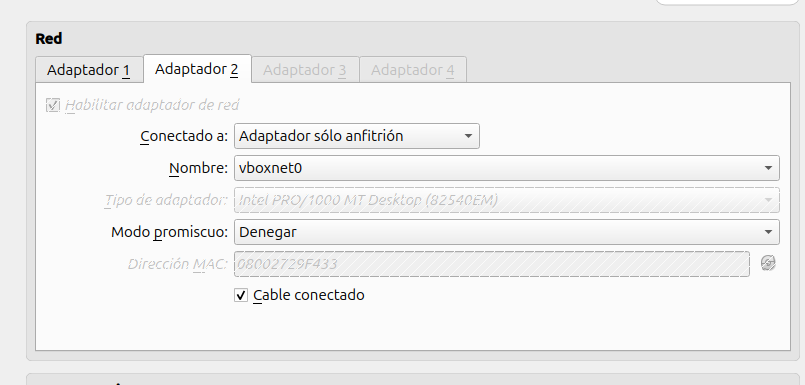
\includegraphics[width=\textwidth]{images/Bloque1/adaptador2.png}
        \caption{Configuración de la red NAT y Host-Only}
    \end{minipage}
    \hfill
    \begin{minipage}[b]{0.45\textwidth}
        \centering
        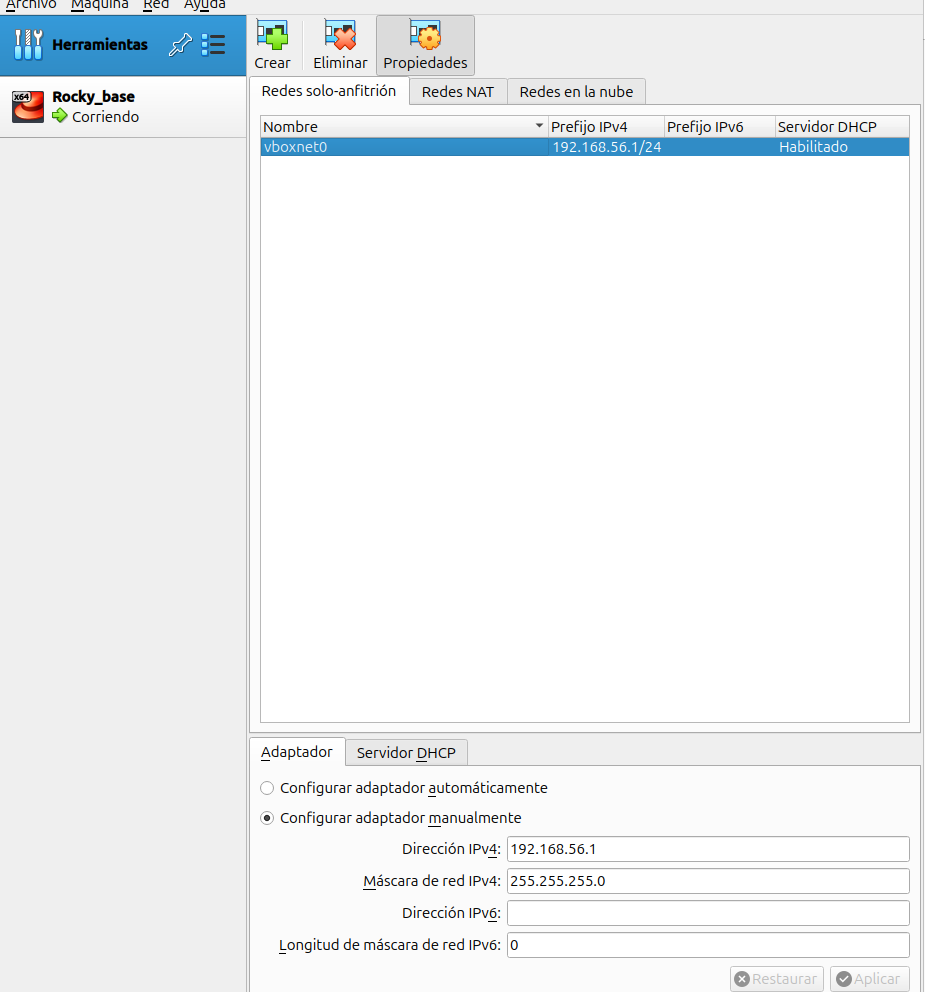
\includegraphics[width=\textwidth]{images/Bloque1/vbox.png}
        \caption{Configuración de VirtualBox para la red de Host-Only}
    \end{minipage}
\end{figure}

Además se nos pide que la Ip de Host Only sea estática, para ello vamos a asegurarnos usando la herramienta \textit{nmtui}, en la que vamos a ver si es estática o no la ip. Como podemos ver en la siguiente imagen esta configurada como ip automática, que viene siendo lo mismo que dinámica por lo que debemos de cambiarlo a manual para poder configurar la ip estática. (Ver Figura 3 y 4). Para ver que efectivamente la ip cambió, podemos verlo en la Figura 5.
\begin{figure}[htbp]
    \centering
    \begin{minipage}[b]{0.45\textwidth}
        \centering
        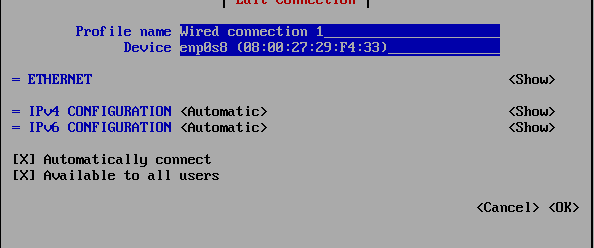
\includegraphics[width=\textwidth]{images/Bloque1/nmtui1.png}
        \caption{Con nmtui vemos que es dinámica}
    \end{minipage}
    \hfill
    \begin{minipage}[b]{0.45\textwidth}
        \centering
        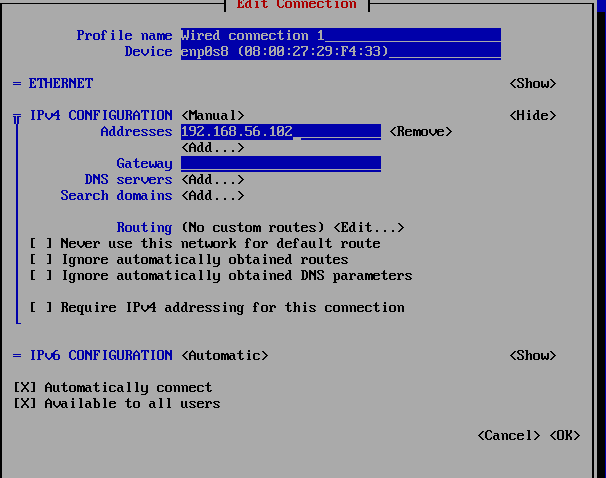
\includegraphics[width=\textwidth]{images/Bloque1/nmtui_2.png}
        \caption{Cambiamos a manual y asignamos una ip estática válida}
    \end{minipage}
\end{figure}



\begin{figure}
    \centering
    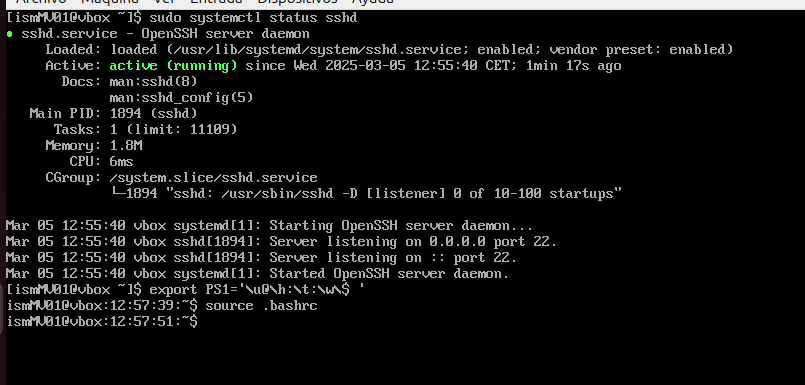
\includegraphics[width=0.8\textwidth]{images/Bloque1/sshd_PS1.png}
    \caption{Sshd y variable PS1}
\end{figure}

\begin{figure}
    \centering
    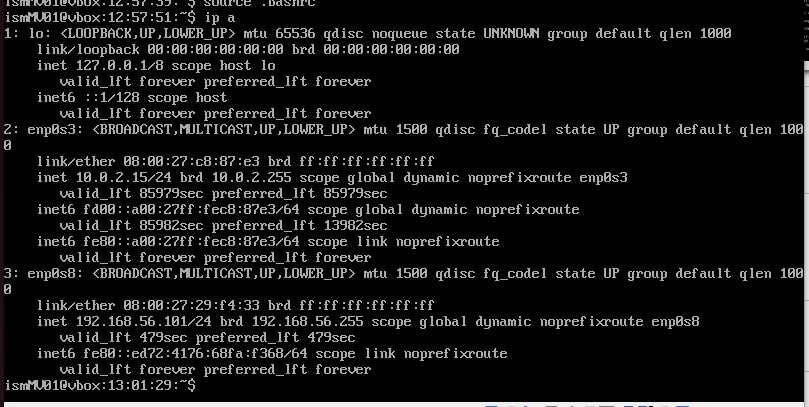
\includegraphics[width=0.8\textwidth]{images/Bloque1/resultado_ipa.png}
    \caption{Resultado de ip a}
\end{figure}

Una vez hayamos cambiado la ip estática, debemos de verificar que efectivamente se ha cambiado y para ello usamos el comando \texttt{ip a} y vemos que efectivamente se ha cambiado la ip a la que hemos asignado. (Ver Figura 7).

\begin{figure}
    \centering
    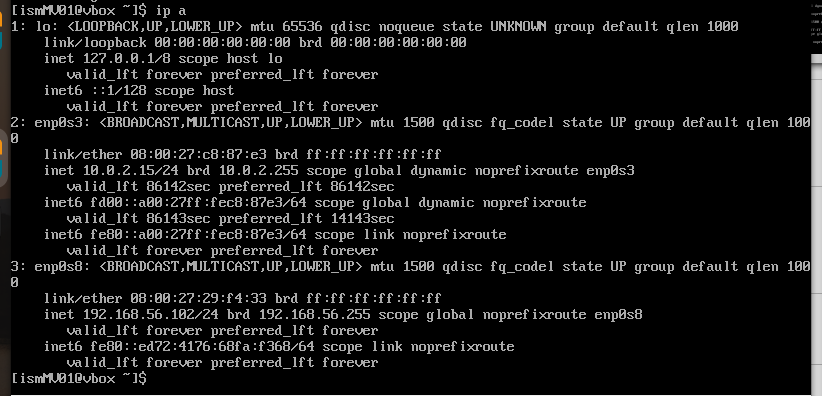
\includegraphics[width=0.8\textwidth]{images/Bloque1/ping2.png}
    \caption{Resultado de ip a para verificar el cambio de ip}
\end{figure}

Llegado a este punto vamos a realizar un ping a la máquina anfitriona y viceversa, para ello usamos el comando \texttt{ping -c <número de pings> ip\_de\_la\_maquina} y vemos que efectivamente hay conexión entre ambas máquinas. (Ver Figura 8, 9 y 10). Además, vemos que gracias al \textit{NAT} podemos hacer ping a cualquier máquina accesible en internet\footnote{Cabe destacar que durante el desarrollo de la actividad, surgían algunas problemas con NetworkManager, polkiy y DBus, pero se solucionaban al reiniciarlos o bien reinstalarlos}. (Ver Figura 11).

\begin{figure}[htbp]
    \centering
    \begin{minipage}[b]{0.45\textwidth}
        \centering
        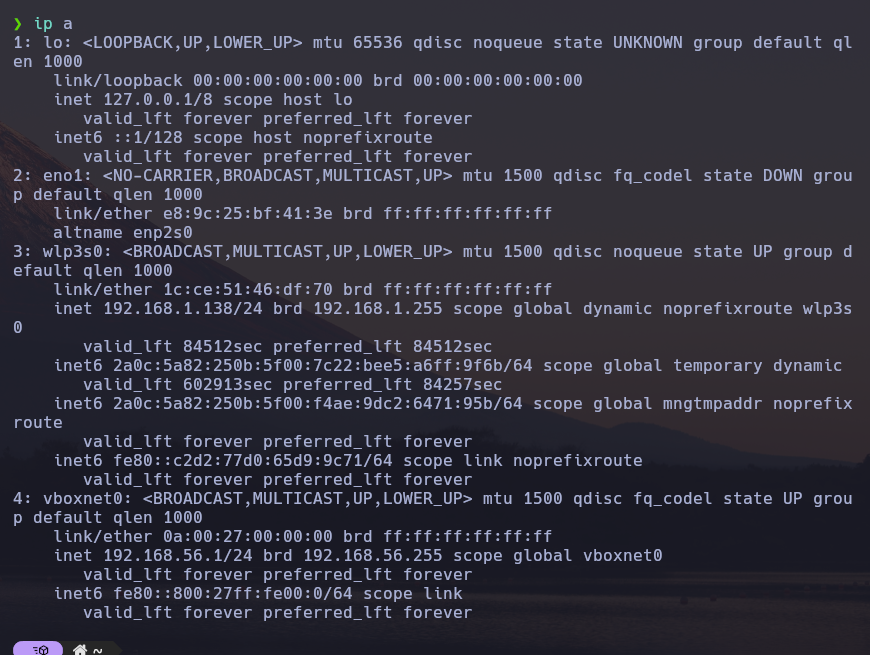
\includegraphics[width=\textwidth]{images/Bloque1/ip_a_host.png}
        \caption{Resultado del comando de \textit{ip a } en la máquina anfitriona para ver la ip}
    \end{minipage}
    \hfill
    \begin{minipage}[b]{0.45\textwidth}
        \centering
        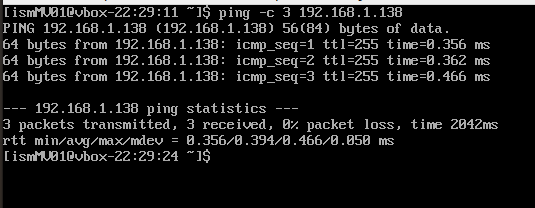
\includegraphics[width=\textwidth]{images/Bloque1/ping_a_anfitriona.png}
        \caption{Ping a la máquina anfitriona}
    \end{minipage}
\end{figure}


\begin{figure}[htbp]
    \centering
    \begin{minipage}[b]{0.45\textwidth}
        \centering
        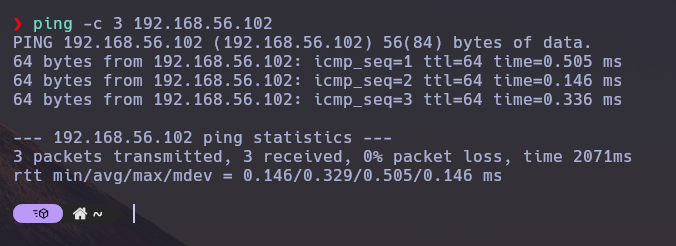
\includegraphics[width=\textwidth]{images/Bloque1/ping_anf_a_mv.png}
        \caption{Ping de la máquina anfitriona a la máquina virtual}
    \end{minipage}
    \hfill
    \begin{minipage}[b]{0.45\textwidth}
        \centering
        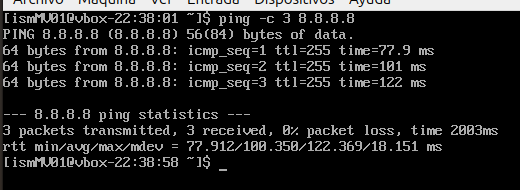
\includegraphics[width=\textwidth]{images/Bloque1/ping_fuera.png}
        \caption{Ping a un servidor público (Google)}
    \end{minipage}
\end{figure}


En cuanto al servicio ssh, debemos de ver el estado del servicio sshd con el comando \texttt{sudo systemctl status sshd} y vemos que esta corriendo. En este punto desde el anfitrión podemos introducirt la línea de comando \texttt{ssh ismMV01@192.168.56.102} y vemos que efectivamente todo funciona correctamente. (Ver Figura 12 y 13).






\begin{figure}[htbp]
    \centering
    \begin{minipage}[b]{0.45\textwidth}
        \centering
        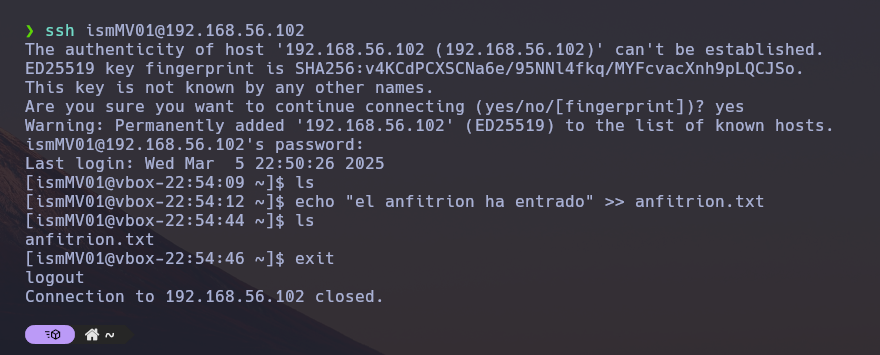
\includegraphics[width=\textwidth]{images/Bloque1/ssh1.png}
        \caption{Ssh en la máquina anfitriona y creación de un archivo en la MV}
    \end{minipage}
    \hfill
    \begin{minipage}[b]{0.45\textwidth}
        \centering
        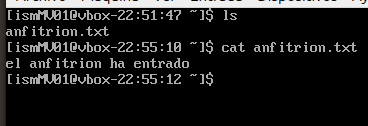
\includegraphics[width=\textwidth]{images/Bloque1/ssh2.png}
        \caption{Ver el contenido del archivo creado en la MV desde el anfitrión}
    \end{minipage}
\end{figure}
\newpage
\section{Servidor con LVM + RAID}

\subsection{Aspectos clave de LVM}

Para gestionar eficazmente el \textit{Logical Volume Manager} (LVM), es fundamental comprender los siguientes componentes y conceptos:

\subsubsection{Componentes de la arquitectura de almacenamiento}

\begin{itemize}
  \item \textbf{Physical Volume (PV)}: Representa los dispositivos de almacenamiento físico, como discos duros o particiones, que se incorporan al sistema LVM.
  \item \textbf{Volume Group (VG)}: Es una agrupación de uno o más PVs que forman un pool de almacenamiento, del cual se pueden asignar espacios para crear volúmenes lógicos.
  \item \textbf{Logical Volume (LV)}: Son volúmenes virtuales creados dentro de un VG. Los LVs se utilizan como si fueran particiones de disco tradicionales, permitiendo la creación de sistemas de archivos o la asignación directa a aplicaciones.
\end{itemize}

\subsubsection{Gestión de almacenamiento con diferentes características físicas}

LVM ofrece flexibilidad para manejar dispositivos de almacenamiento con diversas características físicas:

\begin{itemize}
  \item \textbf{HDD y SSD}: Se pueden combinar en un mismo VG, permitiendo equilibrar rendimiento y capacidad según las necesidades.
  \item \textbf{RAID}: LVM puede trabajar sobre dispositivos RAID, proporcionando una capa adicional de gestión y flexibilidad sobre la configuración RAID existente.
\end{itemize}

\subsubsection{Etiquetado y correspondencia con los archivos de dispositivo}

Cada componente en LVM tiene una nomenclatura específica y se asocia a archivos de dispositivo en el sistema:

\begin{itemize}
  \item \textbf{Physical Volumes}: Corresponden a dispositivos físicos, como \texttt{/dev/sda1}, \texttt{/dev/sdb1}, etc.
  \item \textbf{Volume Groups}: Se nombran según la convención establecida por el administrador, por ejemplo, \texttt{vg\_datos}.
  \item \textbf{Logical Volumes}: Se nombran dentro de su VG correspondiente, como \textit{/dev/vg\_datos/lv\_backup}, donde \textit{lv\_backup} es el nombre del LV.
\end{itemize}

\subsubsection{Comandos de LVM para la gestión de componentes}

LVM proporciona una serie de comandos para administrar sus componentes:

\begin{itemize}
  \item \texttt{pvcreate}: Inicializa un dispositivo físico como PV.
  \item \texttt{vgcreate}: Crea un VG a partir de uno o más PVs.
  \item \texttt{lvcreate}: Crea un LV dentro de un VG.
  \item \texttt{pvs}, \texttt{vgs}, \texttt{lvs}: Muestran información sobre PVs, VGs y LVs respectivamente.
  \item \texttt{pvremove}, \texttt{vgremove}, \texttt{lvremove}: Eliminan PVs, VGs y LVs respectivamente.
\end{itemize}

Estos comandos permiten una gestión eficiente y flexible del almacenamiento en sistemas que utilizan LVM.

\subsection{Niveles de RAID: 0, 1 y 5}

Redundant Array of Independent Disks (RAID) es una tecnología que permite combinar múltiples dispositivos de almacenamiento en una unidad lógica para mejorar el rendimiento, la redundancia o ambos. A continuación, se detallan los niveles de RAID 0, 1 y 5, sus ventajas, desventajas y su administración en sistemas Linux utilizando la herramienta de línea de comandos \texttt{mdadm}.

\subsubsection{RAID 0}

RAID 0, conocido como \textit{striping}, distribuye los datos de manera equitativa entre dos o más discos sin información de paridad ni redundancia.

\begin{itemize}
  \item \textbf{Ventajas}:
    \begin{itemize}
      \item Mayor rendimiento en lectura y escritura debido a la distribución de datos entre los discos.
      \item Uso completo de la capacidad de almacenamiento total, ya que no se reserva espacio para paridad o duplicación.
    \end{itemize}
  \item \textbf{Desventajas}:
    \begin{itemize}
      \item Ausencia de redundancia; la falla de un solo disco resulta en la pérdida total de los datos.
    \end{itemize}
\end{itemize}

\subsubsection{RAID 1}

RAID 1, o \textit{mirroring}, duplica los datos en dos o más discos, creando copias idénticas en cada uno.

\begin{itemize}
  \item \textbf{Ventajas}:
    \begin{itemize}
      \item Alta redundancia; los datos permanecen intactos incluso si uno de los discos falla.
      \item Mejora en la velocidad de lectura, ya que los datos pueden leerse desde cualquiera de los discos.
    \end{itemize}
  \item \textbf{Desventajas}:
    \begin{itemize}
      \item Capacidad de almacenamiento efectiva reducida al 50\% del total, ya que los datos se duplican.
    \end{itemize}
\end{itemize}

\subsubsection{RAID 5}

RAID 5 combina rendimiento y redundancia distribuyendo los datos y la paridad entre tres o más discos.

\begin{itemize}
  \item \textbf{Ventajas}:
    \begin{itemize}
      \item Proporciona tolerancia a fallos; si un disco falla, los datos pueden recuperarse con la información de paridad.
      \item Mejor aprovechamiento del almacenamiento comparado con RAID 1, ya que solo se utiliza una fracción del espacio para la paridad.
    \end{itemize}
  \item \textbf{Desventajas}:
    \begin{itemize}
      \item Rendimiento de escritura inferior al de RAID 0 debido al cálculo de la paridad.
      \item En caso de falla de un disco, la reconstrucción puede ser lenta y afectar el rendimiento.
    \end{itemize}
\end{itemize}

\subsubsection{Administración de RAID en Linux con mdadm}

La herramienta \texttt{mdadm} permite gestionar arreglos RAID en Linux. A continuación, se presentan comandos esenciales:

\begin{itemize}
  \item Crear un RAID 0 con dos discos:
    \begin{lstlisting}[style=mystyle]
    mdadm --create --verbose /dev/md0 --level=0 --raid-devices=2 /dev/sdX /dev/sdY
    \end{lstlisting}
  \item Crear un RAID 1 con dos discos:
    \begin{lstlisting}[style=mystyle]
    mdadm --create --verbose /dev/md0 --level=1 --raid-devices=2 /dev/sdX /dev/sdY
    \end{lstlisting}
  \item Crear un RAID 5 con tres discos:
    \begin{lstlisting}[style=mystyle]
    mdadm --create --verbose /dev/md0 --level=5 --raid-devices=3 /dev/sdX /dev/sdY /dev/sdZ
    \end{lstlisting}
  \item Verificar el estado del RAID:
    \begin{lstlisting}[style=mystyle]
    cat /proc/mdstat
    \end{lstlisting}
  \item Detener un RAID:
    \begin{lstlisting}[style=mystyle]
    mdadm --stop /dev/md0
    \end{lstlisting}
\end{itemize}

\subsection{Aspectos clave para la administración de servidores Linux}

Para implementar eficazmente soluciones en servidores Linux, es esencial comprender y manejar los siguientes aspectos:

\subsubsection{Modos de ejecución y modo de mantenimiento en un servidor Linux}

Los sistemas Linux operan en diferentes niveles de ejecución o \textit{runlevels}, que determinan los servicios y procesos que se ejecutan. Con la adopción de \textit{systemd}, estos niveles se denominan \textit{targets}. El modo de mantenimiento, conocido como \textit{rescue.target} o \textit{emergency.target}, es crucial para tareas de recuperación y administración del sistema. Para cambiar al modo de mantenimiento, se puede utilizar el siguiente comando:

\begin{lstlisting}[style=mystyle]
sudo systemctl isolate rescue.target
\end{lstlisting}

Para volver al modo multiusuario estándar:

\begin{lstlisting}[style=mystyle]
sudo systemctl isolate multi-user.target
\end{lstlisting}

\subsubsection{Estructura estándar del sistema de archivos en Linux}

La estructura de directorios en Linux sigue el estándar de jerarquía de sistemas de archivos (\textit{Filesystem Hierarchy Standard - FHS}). Algunos directorios principales incluyen:

\begin{itemize}
  \item \textbf{/}: Directorio raíz que contiene todos los demás directorios.
  \item \textbf{/bin}: Ejecutables esenciales para todos los usuarios.
  \item \textbf{/etc}: Archivos de configuración del sistema.
  \item \textbf{/home}: Directorios personales de los usuarios.
  \item \textbf{/var}: Datos variables como registros y colas de impresión.
\end{itemize}

\subsubsection{Sistemas de archivos comunes en Linux}

Linux soporta diversos sistemas de archivos. Algunos de los más comunes son:

\begin{itemize}
  \item \textbf{ext4}: Sistema de archivos por defecto en muchas distribuciones, conocido por su estabilidad y rendimiento.
  \item \textbf{XFS}: Adecuado para manejar grandes volúmenes de datos y archivos de gran tamaño.
  \item \textbf{Btrfs}: Ofrece características avanzadas como instantáneas (\textit{snapshots}) y compresión.
\end{itemize}

\subsubsection{Montaje y desmontaje de volúmenes}

El montaje de sistemas de archivos permite acceder a dispositivos de almacenamiento. Para montar un dispositivo:

\begin{lstlisting}[style=mystyle]
sudo mount /dev/sdX1 /mnt/punto_de_montaje
\end{lstlisting}

Para desmontarlo:

\begin{lstlisting}[style=mystyle]
sudo umount /mnt/punto_de_montaje
\end{lstlisting}

Las configuraciones de montaje persistentes se definen en el archivo \texttt{/etc/fstab}.

\subsubsection{Comandos básicos para la gestión de archivos}

La administración de archivos en Linux se realiza mediante comandos de línea. 


% Algunos comandos fundamentales incluyen:

% \begin{itemize}
%   \item \texttt{cp}: Copiar archivos o directorios.
%     \begin{lstlisting}[style=mystyle]
%     cp origen destino
%     \end{lstlisting}
%   \item \texttt{mv}: Mover o renombrar archivos o directorios.
%     \begin{lstlisting}[style=mystyle]
%     mv origen destino
%     \end{lstlisting}
%   \item \texttt{rm}: Eliminar archivos.
%     \begin{lstlisting}[style=mystyle]
%     rm archivo
%     \end{lstlisting}
%   \item \texttt{mkdir}: Crear un nuevo directorio.
%     \begin{lstlisting}[style=mystyle]
%     mkdir nombre_del_directorio
%     \end{lstlisting}
%   \item \texttt{ls}: Listar el contenido de un directorio.
%     \begin{lstlisting}[style=mystyle]
%     ls ruta_del_directorio
%     \end{lstlisting}
%   \item \texttt{cat}: Mostrar el contenido de un archivo.
%     \begin{lstlisting}[style=mystyle]
%     cat archivo
%     \end{lstlisting}
%   \item \texttt{nano} o \texttt{vim}: Editores de texto para modificar archivos desde la terminal.
%     \begin{lstlisting}[style=mystyle]
%     nano archivo
%     \end{lstlisting}
% \end{itemize}

% Estos comandos son esenciales para la gestión diaria de archivos y directorios en un entorno Linux.
Estos se deben de haber estudiado en asignaturas anteriores como Sistemas Operativos.

\subsection{Ejercicio Opcional}

Partiendo de un servidor básico configurado de acuerdo al apartado 2, el alumno/a deberá
afrontar el caso práctico descrito a continuación:

Se desea instalar un servicio de gestión documental en el servidor. Se espera que este servicio
precise de una cantidad espacio de almacenamiento creciente con el tiempo, pudiendo llegar a
ser considerable.

Por otro lado, el contenido será crítico, por lo que se desea proporcionar
algún mecanismo de respaldo ante fallos en el dispositivo de almacenamiento.

El alumno/a debe diseñar los cambios en el sistema de almacenamiento e implementarlo
empleando prácticas adecuadas de administración que garanticen la conservación de la
información en el sistema y procuren la máxima disponibilidad del servicio.

\subsubsection{Solución}

Para la resolución de este ejercicio vamos a seguir lo realizado en clase. (Ver apuntes de clase correspondientes a la sección de LVM+RAID).

En primer lugar creamos los discos, para ello entramos en la configuración de la máquina virtual y añadimos dos discos duros de 1GB cada uno. Una vez añadidos los discos duros, iniciamos la máquina virtual y ejecutamos el comando \texttt{lsblk} para ver los discos duros que tenemos disponibles. (Ver Figura 14).

\begin{figure}[htbp]
  \centering
  \begin{minipage}[b]{0.45\textwidth}
      \centering
      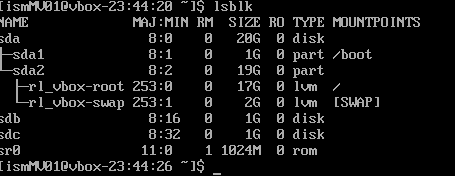
\includegraphics[width=\textwidth]{images/Bloque1/lsblk.png}
      \caption{Resultado del comando lsblk}
  \end{minipage}
  \hfill
  \begin{minipage}[b]{0.45\textwidth}
      \centering
      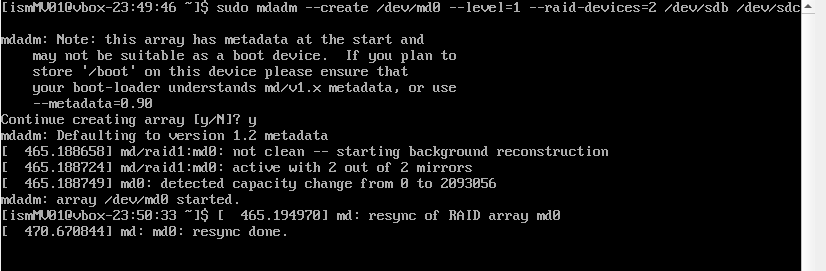
\includegraphics[width=\textwidth]{images/Bloque1/mdadm.png}
      \caption{Comando mdadm}
  \end{minipage}
\end{figure}

A continuación, instalamos \textit{mdadm} con el comando \texttt{sudo dnf install -y mdadm} y creamos un RAID 1 con los dos discos duros que hemos añadido. Para ello ejecutamos el comando \texttt{sudo mdadm --create --verbose /dev/md0 --level=1 --raid-devices=2 /dev/sdb /dev/sdc} y vemos que se ha creado correctamente. (Ver Figura 15).

Acto seguido debemos de crear un PV, VG y LV. Para ello ejecutamos los siguientes comandos (Ver Figura 16):
\begin{itemize}
  \item \texttt{sudo pvcreate /dev/md0}
  \item \texttt{sudo vgcreate vg\_datos /dev/md0}
  \item \texttt{sudo lvcreate -L 900M -n lv\_datos vg\_datos}
\end{itemize}

\begin{figure}[htbp]
  \centering
  \begin{minipage}[b]{0.45\textwidth}
      \centering
      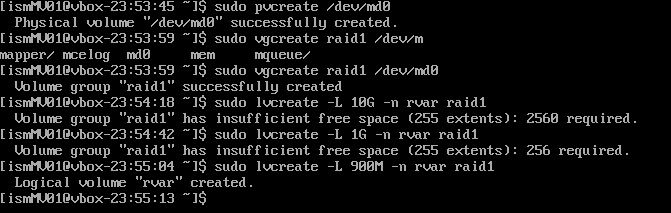
\includegraphics[width=\textwidth]{images/Bloque1/create.png}
      \caption{Resultado de crear los volúmenes}
  \end{minipage}
  \hfill
  \begin{minipage}[b]{0.45\textwidth}
      \centering
      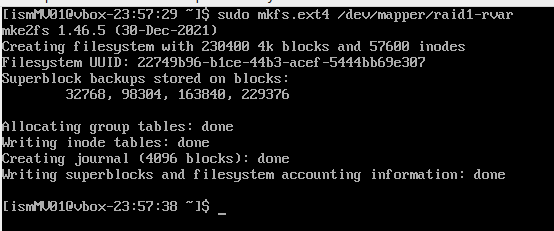
\includegraphics[width=\textwidth]{images/Bloque1/mkfs.png}
      \caption{Comando mkfs}
  \end{minipage}
\end{figure}

Ahora debemos de formatear el volumen lógico en formato ext4. (Ver Figura 17).

A continuación, montamos (Ver Figura 18) y trasladamos la carpeta \textit{var} al nuevo volumen lógico. Para ello ejecutamos los comando que figuran en los apuntes de clase.

\begin{figure}[htbp]
  \centering
  \begin{minipage}[b]{0.45\textwidth}
      \centering
      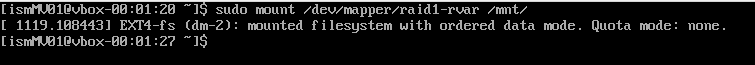
\includegraphics[width=\textwidth]{images/Bloque1/mount.png}
      \caption{Resultado del comando mount}
  \end{minipage}
  \hfill
  \begin{minipage}[b]{0.45\textwidth}
      \centering
      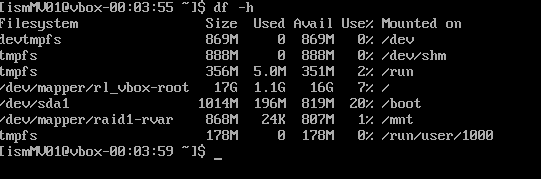
\includegraphics[width=\textwidth]{images/Bloque1/df.png}
      \caption{Comando df -h}
  \end{minipage}
\end{figure}

  Ejecutamos el comando \texttt{df -h} para ver que efectivamente se ha montado correctamente el volumen lógico. (Ver Figura 19).

  Ejecutamos el isolate del systemctl para entrar en modo de mantenimiento y poder trasladar la carpeta \textit{var} al nuevo volumen lógico. (Ver Figura 20).

  \begin{figure}[htbp]
    \centering
    \begin{minipage}[b]{0.45\textwidth}
        \centering
        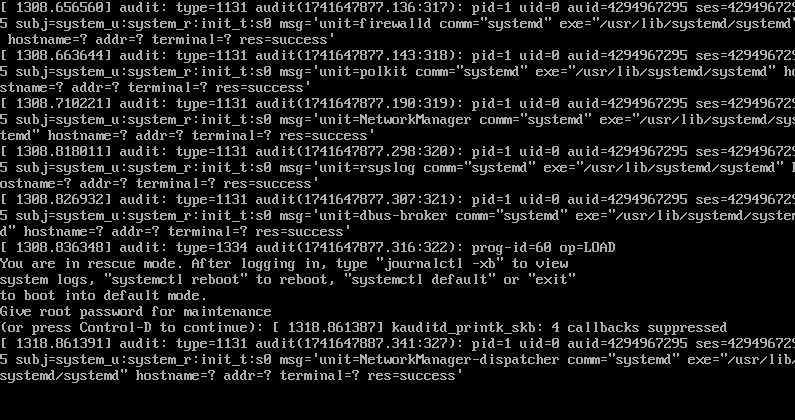
\includegraphics[width=\textwidth]{images/Bloque1/isolate.png}
        \caption{Resultado del comando systemctl isolate}
    \end{minipage}
    \hfill
    \begin{minipage}[b]{0.45\textwidth}
        \centering
        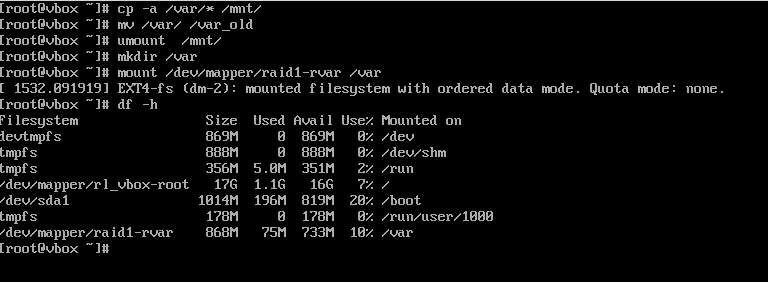
\includegraphics[width=\textwidth]{images/Bloque1/var.png}
        \caption{Serie de operaciones para trasladar la carpeta var}
    \end{minipage}
  \end{figure}

Ahora debemos de trabajar con la serie de comandos que se especifican para poder mover la carpeta y que se haga de forma correcta. (Ver Figura 21).

Una vez trasladad la carpeta, debemos de hacer permanentes los cambios, para ello debemos de editar el fichero \texttt{/etc/fstab} y añadir la siguiente línea (Ver Figura 22):

\begin{lstlisting}[style=mystyle]
  /dev/mapper/raid1-rvar /var ext4 defaults 0 0
\end{lstlisting}

Recargamos la configuraciones con el deamon de systemd y vemos que aparece la parte que estabamos montando (Ver Figura 23).

\begin{figure}[htbp]
  \centering
  \begin{minipage}[b]{0.45\textwidth}
      \centering
      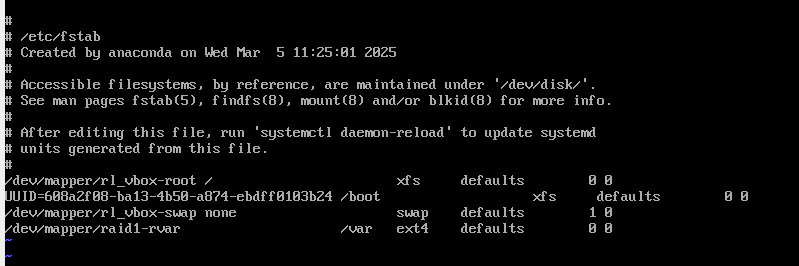
\includegraphics[width=\textwidth]{images/Bloque1/fstab.png}
      \caption{Resultado de editar /etc/fstab como se indica}
  \end{minipage}
  \hfill
  \begin{minipage}[b]{0.45\textwidth}
      \centering
      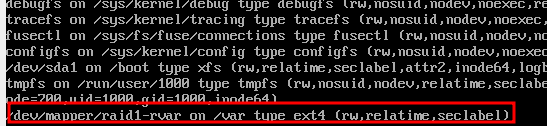
\includegraphics[width=\textwidth]{images/Bloque1/daemon.png}
      \caption{Resultado del comando systemctl daemon-reload y mount}
  \end{minipage}
\end{figure}

Y como podemos comprobar en la Figura 24, hemos conseguido trasladar la carpeta \textit{var} al nuevo volumen lógico y todo funciona correctamente.

\begin{figure}[H]
  \centering
  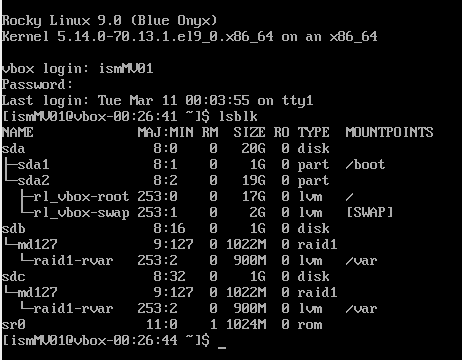
\includegraphics[width=0.6\textwidth]{images/Bloque1/resultadofinal_raid.png}
  \caption{Resultado final}
\end{figure}

\newpage
\section{Acceso seguro al servidor: Firewall + SSHD}

\subsection{Iptables}

\texttt{iptables} es una herramienta de línea de comandos utilizada para configurar el cortafuegos en el núcleo de Linux, implementado dentro del proyecto Netfilter. Aunque \texttt{iptables} es un marco heredado, \texttt{nftables} se presenta como su reemplazo moderno, ofreciendo una capa de compatibilidad. 

\subsubsection{Instalación}

El núcleo estándar de Arch Linux viene compilado con soporte para \texttt{iptables}. Para instalar las utilidades de usuario, se debe instalar el paquete \texttt{iptables}, que es una dependencia indirecta del metapaquete \texttt{base}, por lo que debería estar instalado por defecto en el sistema. 

\subsubsection{Conceptos Básicos}

\begin{itemize}
    \item \textbf{Tablas}: Colecciones de reglas con propósitos específicos.
    \item \textbf{Cadenas}: Listas de reglas dentro de una tabla que se recorren en orden.
    \item \textbf{Reglas}: Definiciones que consisten en un criterio de coincidencia y una acción a ejecutar si se cumple dicho criterio.
\end{itemize}

\subsubsection{Configuración y Uso}

\texttt{iptables} se puede configurar directamente desde la línea de comandos o mediante diversas interfaces frontales, tanto de consola como gráficas. Para mostrar las reglas actuales, se utiliza:

\begin{verbatim}
iptables -L
\end{verbatim}

Para restablecer las reglas:

\begin{verbatim}
iptables -F
\end{verbatim}

\subsubsection{Registro de Actividad}

\texttt{iptables} permite registrar paquetes para monitorear actividad o depurar reglas. Es posible limitar la tasa de registro para evitar la saturación de los registros del sistema. 
\subsubsection{Alternativas y Herramientas Relacionadas}

\begin{itemize}
    \item \textbf{\texttt{nftables}}: Proyecto que busca reemplazar a \texttt{iptables}, proporcionando un nuevo marco de filtrado de paquetes y una utilidad de espacio de usuario llamada \texttt{nft}. 
    \item \textbf{\texttt{ipset}}: Aplicación complementaria que permite crear conjuntos de direcciones IP para ser utilizados en reglas de \texttt{iptables}, facilitando el bloqueo o la aceptación de múltiples direcciones de manera eficiente. 
    \item \textbf{\texttt{ufw} (Uncomplicated Firewall)}: Programa para gestionar el cortafuegos de manera sencilla, proporcionando una interfaz de línea de comandos fácil de usar. 
\end{itemize}

\subsubsection{Recursos Adicionales}

Para configuraciones más avanzadas, como la creación de un cortafuegos con estado o compartir la conexión a Internet, se pueden consultar las siguientes guías:

\begin{itemize}
    \item \textbf{Cortafuegos con Estado Sencillo}: Explica cómo configurar un cortafuegos con estado utilizando \texttt{iptables}, detallando las reglas necesarias y su propósito. 
    \item \textbf{Compartir Conexión a Internet}: Describe cómo compartir la conexión a Internet desde una máquina a otras, incluyendo los requisitos y pasos necesarios.
\end{itemize}


\subsection{firewalld y firewall-cmd en Rocky Linux}

\texttt{firewalld} es un servicio de cortafuegos dinámico que permite gestionar reglas de firewall sin necesidad de reiniciar el servicio. Su herramienta de línea de comandos, \texttt{firewall-cmd}, proporciona una interfaz para la administración del firewall en sistemas como Rocky Linux.

\subsubsection{Gestión del Firewall con firewall-cmd}

\texttt{firewall-cmd} permite configurar reglas de firewall de manera flexible y en tiempo real. Algunas de las operaciones más comunes incluyen:

\begin{itemize}
    \item \textbf{Verificar el estado del firewall}:
    \begin{verbatim}
    firewall-cmd --state
    \end{verbatim}

    \item \textbf{Listar las reglas activas}:
    \begin{verbatim}
    firewall-cmd --list-all
    \end{verbatim}

    \item \textbf{Abrir un puerto específico} (ejemplo: puerto 80 TCP):
    \begin{verbatim}
    firewall-cmd --add-port=80/tcp --permanent
    \end{verbatim}
    
    \item \textbf{Cerrar un puerto específico}:
    \begin{verbatim}
    firewall-cmd --remove-port=80/tcp --permanent
    \end{verbatim}

    \item \textbf{Recargar la configuración del firewall} para aplicar cambios:
    \begin{verbatim}
    firewall-cmd --reload
    \end{verbatim}
\end{itemize}

\subsubsection{Administración del Servicio firewalld con systemctl}

\texttt{systemctl} es una herramienta utilizada para gestionar servicios en sistemas basados en \texttt{systemd}, como Rocky Linux. Se puede utilizar para controlar el servicio \texttt{firewalld} de la siguiente manera:

\begin{itemize}
    \item \textbf{Verificar si el servicio está activo}:
    \begin{verbatim}
    systemctl status firewalld
    \end{verbatim}

    \item \textbf{Iniciar el servicio} si está detenido:
    \begin{verbatim}
    systemctl start firewalld
    \end{verbatim}

    \item \textbf{Detener el servicio} si se necesita desactivarlo temporalmente:
    \begin{verbatim}
    systemctl stop firewalld
    \end{verbatim}

    \item \textbf{Habilitar el servicio para que se inicie automáticamente} al arrancar el sistema:
    \begin{verbatim}
    systemctl enable firewalld
    \end{verbatim}

    \item \textbf{Deshabilitar el servicio para evitar su inicio automático}:
    \begin{verbatim}
    systemctl disable firewalld
    \end{verbatim}
\end{itemize}

\subsubsection{Verificación de Configuración con nmap}

\texttt{nmap} es una herramienta de escaneo de redes que permite verificar los puertos abiertos y configuraciones de firewall. Se puede usar para comprobar la efectividad de las reglas de firewall aplicadas. Algunos ejemplos de uso incluyen:

\begin{itemize}
    \item \textbf{Escanear los puertos abiertos de una dirección IP específica}:
    \begin{verbatim}
    nmap <direccion_ip>
    \end{verbatim}

    \item \textbf{Escanear puertos específicos} (ejemplo: puertos 22 y 80):
    \begin{verbatim}
    nmap -p 22,80 <direccion_ip>
    \end{verbatim}

    \item \textbf{Detectar el sistema operativo del host analizado}:
    \begin{verbatim}
    nmap -O <direccion_ip>
    \end{verbatim}
\end{itemize}

Estas herramientas permiten una administración avanzada del firewall en Rocky Linux, garantizando la seguridad de la red y el control del tráfico de red en el sistema.

\subsection{Ejercicio Opcional}

Como caso práctico, partiendo de una MV con la configuración base descrita en el apartado 2, el
alumno/a deberá ser capaz de instalar un servidor de HTTP, Apache o Nginx,
y habilitar/deshabilitar su acceso por Firewall.

Para ello, instalará el servidor web de su elección y modificará la home page para mostrar un
mensaje:'Bienvenidos a la web de <Nombre y Apellidos del alumno/a> en Prácticas ISE'.

El servicio web debe estar accesible en la servidor (MV) en el puerto por defecto (80) usando un
navegador web convencional corriendo en el anfitrión (Host).

Un escaneo de puertos sobre el servidor solo debe mostrar como accesibles los puerto web y ssh.

\subsection*{Solución}

Para la resolución de este ejercicio vamos a seguir los siguientes pasos:

\begin{enumerate}
\item Instalamos el servidor web Apache con el comando \micode{sudo dnf install -y httpd}. También tenemos la opción de instalar Nginx con el comando \micode{sudo dnf install nginx- y}. \textit{Tenemos libre elección de servidor web, en mi caso será Apache}.
\item Debemos de activar este servicio con el comando:
  \begin{itemize}
    \item Apache: \micode{sudo systemctl enable httpd --now}
    \item Nginx: \micode{sudo systemctl enable nginx --now}
    \item Debemos de verificar que el servicio esta activo con los comandos:
    \begin{itemize}
      \item \micode{sudo systemctl status httpd # Para Apache}
      \item \micode{sudo systemctl status nginx # Para Nginx}
    \end{itemize}
  \end{itemize}
  \item Modificación de la página principal.\\
  Debemos de personalizar la página de inicio de nuestra web para que muestre el mensaje que se nos pide en el enunciado.
  \begin{itemize}
    \item Apache: \micode{echo "Bienvenidos a la web de <Nombre y Apellidos> en Prácticas ISE" | sudo tee /var/www/html/index.html}
    \item Nginx: \micode{echo "Bienvenidos a la web de <Nombre y Apellidos> en Prácticas ISE" | sudo tee /usr/share/nginx/html/index.html}
  \end{itemize}
  \item Configuración del Firewall.\\
  Para permitir el acceso a la web, es necesario abrir el puerto 80 en el firewall. Para ello, ejecutamos los siguientes comandos:
  \begin{itemize}
    \item \micode{sudo firewall-cmd --add-service=http --permanent}
    \item \micode{sudo firewall-cmd --reload}
    \item Para verificar que el puerto esta abierto: \micode{sudo firewall-cmd --list-all}
  \end{itemize}
  \item Acceder desde el Navegador.\\
  Si todo está configurado correctamente, se visualizará el mensaje personalizado\footnote{Para saber a que ip acceder, podemos usar el comando \textit{ip a} y coger la correspondiente a \textit{enp0s8.}}(Ver Figura \ref{web}).
  \begin{figure}[H]
    \centering
      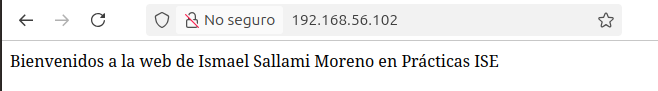
\includegraphics[width=0.7\textwidth]{images/Bloque1/web.png}
      \caption{Acceso a la web desde el navegador}
      \label{web}
  \end{figure}
  \item Restricción de puertos con Firewall.\\
  Para asegurar que solo los puertos web (80) y SSH (22) estén accesibles, se deben eliminar
otras reglas de firewall:
\begin{itemize}
  \item \micode{sudo firewall-cmd --list-services --permanent}\footnote{Con este comando podemos ver los servicios que están activos en el firewall, desactivamos todos, a excepción de http y ssh.}
  \item \micode{sudo firewall-cmd --remove-service=<nombre> --permanent}
  \item \micode{sudo firewall-cmd --reload}
  \item Extra.\\
  Como extra podemos ver los puertos que están abiertos con el comando \micode{sudo firewall-cmd --list-ports --permanent} y cerramos el puerto con \micode{sudo firewall-cmd --remove-port=xxxx/tcp --permanent}, donde xxxx es el puerto que queremos cerrar. Otra forma de solo tener dos puertos abiertos es con los comandos:
  \begin{itemize}
    \item \micode{sudo firewall-cmd --add-service=http --permanent}
    \item \micode{sudosudo firewall-cmd --add-service=ssh --permanent}
    \item Y de nuevo recargamos y listamos todos los puertos.
  \end{itemize}
\end{itemize}
\end{enumerate}

\newpage
\section{SSH}

\subsection{Administración remota con SSH y criptografía asimétrica}

La administración remota es una tarea fundamental en la gestión de servidores. Una de las herramientas más utilizadas para este propósito es \texttt{SSH} (Secure Shell), que permite acceder y administrar un sistema de manera segura a través de una red. Es importante destacar que \texttt{SSH} puede referirse tanto a un cliente como a un servicio.

\subsubsection{Instalación y configuración de SSH}
Para instalar y habilitar el servicio SSH en un sistema basado en Rocky Linux, se utilizan los siguientes comandos:

\begin{lstlisting}[style=mystyle]
sudo dnf install -y openssh-server
sudo systemctl enable --now sshd
\end{lstlisting}

El servicio \texttt{sshd} es el demonio que permite las conexiones SSH entrantes. Su configuración se encuentra en el archivo:

\begin{lstlisting}[style=mystyle]
/etc/ssh/sshd_config
\end{lstlisting}

Al editar este archivo, es posible modificar diversas opciones de seguridad, como:

\begin{itemize}
    \item \textbf{Deshabilitar el acceso como root por contraseña:} Para mejorar la seguridad, se recomienda restringir el acceso directo de root:
    \begin{lstlisting}[style=mystyle]
    PermitRootLogin no
    \end{lstlisting}
    
    \item \textbf{Cambio de puerto predeterminado:} SSH por defecto usa el puerto 22, pero puede cambiarse para reducir ataques automatizados:
    \begin{lstlisting}[style=mystyle]
    Port 2222
    \end{lstlisting}
\end{itemize}

Después de modificar la configuración, es necesario reiniciar el servicio:

\begin{lstlisting}[style=mystyle]
sudo systemctl restart sshd
\end{lstlisting}

\subsubsection{Configuración del firewall para SSH}
Si se cambia el puerto de \texttt{SSH}, es necesario actualizar la configuración del firewall:

\begin{lstlisting}[style=mystyle]
sudo firewall-cmd --add-port=2222/tcp --permanent
sudo firewall-cmd --reload
\end{lstlisting}

\subsubsection{Criptografía simétrica y asimétrica en SSH}
\textbf{Criptografía simétrica} es un método en el que la misma clave se usa tanto para cifrar como para descifrar los datos. Es rápida pero menos segura para la comunicación remota, ya que ambas partes deben compartir la clave de forma segura.

\textbf{Criptografía asimétrica}, utilizada en SSH, emplea un par de claves: una clave pública y una clave privada. El cliente genera un par de claves y comparte la clave pública con el servidor, lo que permite autenticarse sin necesidad de enviar una contraseña.

Para generar un par de claves en SSH, se usa:

\begin{lstlisting}[style=mystyle]
ssh-keygen -t rsa -b 4096
\end{lstlisting}

Y para copiar la clave pública al servidor:

\begin{lstlisting}[style=mystyle]
ssh-copy-id usuario@servidor
\end{lstlisting}

Esto permite autenticarse sin necesidad de contraseña, mejorando la seguridad y facilitando la automatización de tareas en servidores remotos.

\subsection{Ejercicio Opcional}

Partiendo de un servidor base configurado siguiendo las indicaciones del apartado 2, el
alumno/a modificará servicio SSHD para que, en lugar del puerto por defecto (22), se ejecute en
un puerto alternativo de un valor mayor a 1024. Se recomienda que consulte la lista de puertos
reconocidos por el sistema en /etc/ports para evitar emplear un puerto que ya tenga una
aplicación predefinida.

Se concederá acceso remoto por llave pública a un usuario de su elección.
El ejercicio se validará ejecutando un comando de forma remota sobre el servidor SSH con la
nueva configuración. El comando presentará el contenido completo (incluido ficheros y
directorios ocultos) con del directorio home del usuario remoto empleado en la conexión. Para
ello, desde el ordenador anfitrión (o una MV distinta a la que se va a acceder) se empleará ssh
sin terminal remoto y sin contraseña, pasando como único como parámetro el comando a
ejecutar.

\subsection*{Solución}

\subsection*{Modificación del servicio SSHD y acceso remoto por llave pública}

En este ejercicio, se modificará la configuración del servicio SSH para que utilice un puerto alternativo y se habilitará el acceso remoto mediante autenticación con clave pública.

\subsubsection*{Paso 1: Verificar puertos disponibles}

Antes de modificar la configuración de SSH, es recomendable consultar la lista de puertos reconocidos por el sistema para evitar conflictos con otros servicios. Para ello, se puede inspeccionar el archivo:

\begin{lstlisting}[style=mystyle]
cat /etc/services | less
\end{lstlisting}

Se debe elegir un puerto mayor a 1024 que no esté en uso.

\subsubsection*{Paso 2: Modificar la configuración de SSH}

Editar el archivo de configuración de SSH con un editor de texto como `vim` o `nano`:

\begin{lstlisting}[style=mystyle]
sudo nano /etc/ssh/sshd_config
\end{lstlisting}

Buscar la línea que especifica el puerto (`\#Port 22`), descomentarla y cambiarla por el número de puerto elegido, por ejemplo:

\begin{lstlisting}[style=mystyle]
Port 2222
\end{lstlisting}

Guardar los cambios y salir del editor.

\subsubsection{Solución al error al cambiar el puerto de SSH}

Si al cambiar el puerto en la configuración de SSH y reiniciar el servicio se obtiene un error, se deben seguir los siguientes pasos para solucionar el problema:

\begin{enumerate}
    \item \textbf{Verificar errores en la configuración de SSH}  
    Ejecutar el siguiente comando para comprobar si hay errores en el archivo de configuración:

    \begin{lstlisting}[style=mystyle]
    sudo sshd -t
    \end{lstlisting}

    Si se detectan errores de sintaxis o configuración en el archivo \textit{/etc/ssh/sshd\_config}, se deben corregir antes de continuar.

    \item \textbf{Confirmar que el puerto está permitido en SELinux (si aplica)}  
    Si el sistema usa SELinux, es necesario permitir el nuevo puerto:

    \begin{lstlisting}[style=mystyle]
    sudo semanage port -a -t ssh_port_t -p tcp 2222
    \end{lstlisting}

    Si el comando \texttt{semanage} no está disponible, se puede instalar con:

    \begin{lstlisting}[style=mystyle]
    sudo dnf install policycoreutils-python-utils
    \end{lstlisting}

    Luego, verificar que el puerto se agregó correctamente con:

    \begin{lstlisting}[style=mystyle]
    sudo semanage port -l | grep ssh
    \end{lstlisting}

    \item \textbf{Permitir el nuevo puerto en \texttt{firewalld}}  
    Si el sistema usa \texttt{firewalld}, se debe agregar el puerto y recargar la configuración:

    \begin{lstlisting}[style=mystyle]
    sudo firewall-cmd --permanent --add-port=2222/tcp
    sudo firewall-cmd --reload
    \end{lstlisting}

    \item \textbf{Reiniciar el servicio SSH y comprobar su estado}  
    Una vez realizados los cambios, reiniciar el servicio SSH:

    \begin{lstlisting}[style=mystyle]
    sudo systemctl restart sshd
    \end{lstlisting}

    Si el servicio sigue fallando, revisar los logs para obtener más detalles sobre el error:

    \begin{lstlisting}[style=mystyle]
    sudo journalctl -xeu sshd
    \end{lstlisting}
\end{enumerate}

Siguiendo estos pasos, se podrá cambiar el puerto de SSH sin problemas y reiniciar el servicio correctamente.


\subsubsection*{Paso 3: Ajustar firewalld para permitir conexiones en el nuevo puerto}

Si `firewalld` está en uso, es necesario agregar el nuevo puerto al firewall y eliminar el acceso al puerto 22 si no se desea que permanezca abierto:

\begin{lstlisting}[style=mystyle]
sudo firewall-cmd --permanent --add-port=2222/tcp
sudo firewall-cmd --permanent --remove-service=ssh
sudo firewall-cmd --reload
\end{lstlisting}

\subsubsection*{Paso 4: Reiniciar el servicio SSH}

Aplicar los cambios reiniciando el servicio SSH:

\begin{lstlisting}[style=mystyle]
sudo systemctl restart sshd
\end{lstlisting}

\subsubsection*{Paso 5: Configurar autenticación por clave pública}

Desde el cliente, generar un par de claves SSH si no se tienen:

\begin{lstlisting}[style=mystyle]
ssh-keygen -t rsa -b 4096
\end{lstlisting}

Copiar la clave pública al servidor(Ver Figura \ref{copiaLlave}):

\begin{lstlisting}[style=mystyle]
ssh-copy-id -p 2222 usuario@IP_del_Servidor
\end{lstlisting}

\begin{figure}[H]
  \centering
  \begin{minipage}[b]{0.45\textwidth}
    \centering
    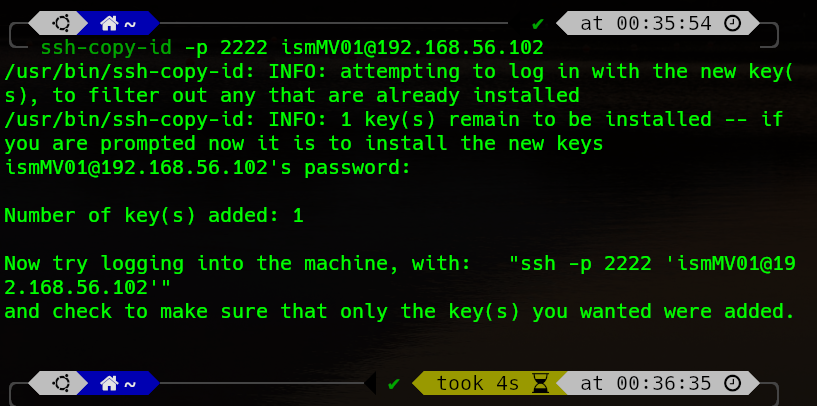
\includegraphics[width=\textwidth]{images/copiaLlave.png}
    \caption{SSH en mi máquina}
    \label{copiaLlave}
  \end{minipage}
  \hfill
  \begin{minipage}[b]{0.45\textwidth}
    \centering
    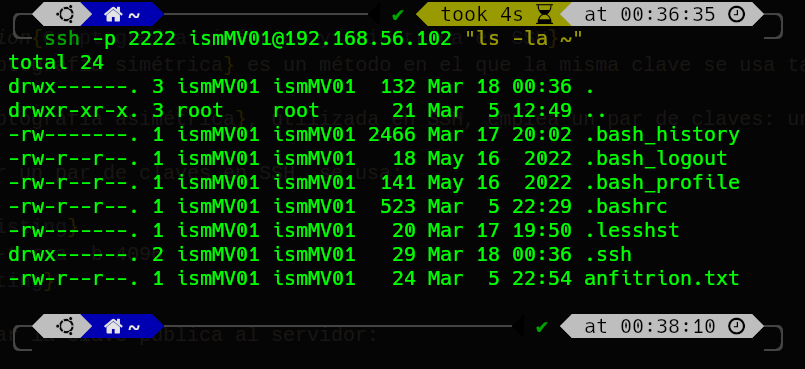
\includegraphics[width=\textwidth]{images/finalSSH.png}
    \caption{SSH final}
    \label{finalSSH}
  \end{minipage}
\end{figure}

\subsubsection*{Paso 6: Validar la conexión sin contraseña}

Para comprobar que el acceso es correcto, se ejecutará un comando remoto en la máquina virtual desde otro equipo o una máquina anfitriona. Se listará el contenido completo del directorio home del usuario remoto, incluidos los archivos ocultos (Ver Figura \ref{finalSSH}):

\begin{lstlisting}[style=mystyle]
ssh -p 2222 usuario@IP_del_Servidor "ls -la ~"
\end{lstlisting}

Si todo está configurado correctamente, el comando mostrará los archivos del directorio home sin requerir contraseña.

\newpage
\section{Automatización de la configuración con Ansible}

\subsection{Introducción a Ansible}

Ansible es una herramienta de automatización que permite gestionar configuraciones y despliegues en múltiples sistemas de manera sencilla y eficiente. Su funcionamiento se basa en la ejecución de comandos remotos a través de SSH y utiliza Python como lenguaje de scripting, lo que facilita su integración en la mayoría de las distribuciones Linux.

\subsubsection{Comandos Ad-Hoc en Ansible}

Los comandos ad-hoc en Ansible permiten ejecutar tareas únicas y rápidas en uno o varios nodos gestionados sin necesidad de crear un playbook. Se utilizan a través de la herramienta de línea de comandos \texttt{ansible} y son ideales para operaciones puntuales, como reiniciar servicios, copiar archivos o instalar paquetes. Aunque son fáciles de usar, no son reutilizables ni idempotentes, por lo que para tareas repetitivas o complejas se recomienda el uso de playbooks. \cite{turn0search0}

\subsubsection{Módulos de Ansible}

Ansible cuenta con una amplia variedad de módulos que encapsulan tareas específicas, como gestionar usuarios, instalar paquetes o manejar servicios. Estos módulos permiten abstraer la complejidad de las operaciones subyacentes y proporcionan una interfaz consistente para interactuar con diferentes sistemas y servicios. La documentación oficial de Ansible ofrece un índice completo de todos los módulos disponibles, organizados por categorías, facilitando la búsqueda y selección del módulo adecuado para cada tarea. \cite{turn0search4}

\subsubsection{Playbooks en Ansible}

Los playbooks son el núcleo de Ansible y permiten definir configuraciones, despliegues y orquestaciones de manera declarativa y reproducible. Están escritos en formato YAML y constan de una o más 'plays', cada una de las cuales especifica un conjunto de tareas a ejecutar en un grupo de hosts. Los playbooks pueden:

\begin{itemize}
    \item Declarar configuraciones de sistemas.
    \item Orquestar procesos manuales en múltiples máquinas en un orden definido.
    \item Ejecutar tareas de forma síncrona o asíncrona.
\end{itemize}

Al escribir playbooks, es esencial comprender su sintaxis y estructura para garantizar su correcta ejecución y mantenimiento. \cite{turn0search2}

\subsubsection{Buenas Prácticas de Seguridad}

Es una práctica recomendada en Ansible evitar el uso del usuario 'root' para acceder a los nodos gestionados. En su lugar, se aconseja crear un usuario con privilegios adecuados que se conecte mediante SSH utilizando autenticación con clave pública y que pueda ejecutar comandos privilegiados sin necesidad de ingresar una contraseña adicional. Para ello, es necesario configurar correctamente el comando \texttt{sudo} en el servidor, permitiendo que el usuario tenga los permisos necesarios para las operaciones requeridas.

\subsubsection{Administración del Inventario}

El inventario en Ansible es un archivo que define los hosts y grupos de hosts sobre los cuales se ejecutarán las tareas. Es fundamental para organizar y gestionar los nodos de manera eficiente. Ansible permite utilizar inventarios estáticos, definidos en archivos de texto, o dinámicos, generados por scripts que consultan fuentes externas. Una correcta administración del inventario facilita la segmentación de los hosts y la aplicación de configuraciones específicas a diferentes grupos de servidores.

\subsubsection{Ejecución de Comandos Ad-Hoc por CLI}

Además de los playbooks, Ansible permite la ejecución de comandos ad-hoc directamente desde la línea de comandos. Esta funcionalidad es útil para tareas rápidas y únicas, como verificar el estado de un servicio o copiar un archivo a múltiples servidores. Aunque los comandos ad-hoc son prácticos, para tareas más complejas o repetitivas se recomienda encapsular las operaciones en playbooks para asegurar la reproducibilidad y el mantenimiento del código.

\subsubsection{Configuración de Servidores con Playbooks}

Los playbooks permiten automatizar la configuración de servidores de manera declarativa. Al definir el estado deseado de los sistemas, Ansible se encarga de aplicar las tareas necesarias para alcanzar ese estado. Esto incluye la instalación y configuración de paquetes, la gestión de archivos y servicios, y la implementación de políticas de seguridad. La utilización de playbooks facilita la gestión coherente y reproducible de las configuraciones en múltiples servidores, reduciendo errores y mejorando la eficiencia operativa.


\subsection{Ejercicio Obligatorio}

El ejercicio versa sobre la configuración de servidores empleando Ansible playbooks. Se valorará la estructuración y claridad del código, el uso de parámetros para facilitar la reutilización de los playbooks, el uso de comentarios, el uso de variables, la organización de los artefactos, el uso de convenciones de nombrado de Ansible y de Yaml y, aunque escapa al objetivo de este ejercicio, el posible uso de recursos para reutilización de artefactos, como los Ansible Roles.

Partiendo de dos servidores, configurados de acuerdo a los requerimientos del apartado 2, debe modificarlos para que sea posible el acceso remoto del usuario root empleando contraseña (el acceso con contraseña está desactivado por defecto en la instalación de Rocky).

A continuación, realizará la siguiente configuración en los dos servidores empleando un playbook:
\begin{enumerate}
  \item Crear un nuevo usuario llamado “admin” que pueda ejecutar comandos privilegiados sin contraseña.
  \item Dar acceso por SSH al usuario “admin” con llave pública.
  \item Crear el grupo “wheel” (si no existe) y permitir a sus miembros ejecutar sudo.
  \item Añadir una lista variable de usuarios (se proporcionará un ejemplo con al menos dos), añadiéndolos al grupo “wheel” y concediéndoles acceso por SSH con llave pública.
  \item Deshabilitar el acceso por contraseña sobre SSH para el usuario root.
\end{enumerate}

Los servidores anteriormente configurados son ahora administrables mediante Ansible empleando el usuario “admin”. Ponga a prueba esta configuración con los siguientes cambios/playbooks:
\begin{enumerate}
  \item Modifique convenientemente el inventario para el uso del nuevo usuario “admin”.
  \item Uno de los servidores se empleará para correr Apache Httpd y el otro Nginx. Modifique el inventario de forma conveniente para realizar correctamente su administración.
  \item Desarrolle un playbook para implementar los requerimientos del ejercicio 4.1.1 en los dos servidores, instalando en cada caso Apache Httpd o Nginx según la configuración del inventario.
\end{enumerate}

Todos los archivos necesarios para la ejecución de los Playbooks (playbooks, inventario, variables, scripts, …) deben estar localizados en un directorio (con posibles subdirectorios). Junto a los archivos propios de Ansible, debe proporcionar dos scripts (por ejemplo, \texttt{iniciarNodosManejados.sh} y \texttt{configurarWebServers.sh}) para la ejecución de los playbooks con todos los parámetros necesarios.

% \begin{verbatim}
% # Estructura del directorio para los playbooks y scripts
% project_directory/
% |-- inventory.ini
% |-- group_vars/
% |   |-- all.yml
% |   |-- apache.yml
% |   `-- nginx.yml
% |-- playbooks/
% |   |-- initial_setup.yml
% |   `-- webserver_setup.yml
% |-- scripts/
% |   |-- iniciarNodosManejados.sh
% |   `-- configurarWebServers.sh
% `-- files/
%     |-- admin_ssh_key.pub
%     `-- users_ssh_keys/
%         |-- user1.pub
%         `-- user2.pub
% \end{verbatim}

% Example usage
\begin{directorylisting}[Estructura del directorio para los playbooks y scripts]
  project_directory/
  |-- inventory.ini
  |-- group_vars/
  |   |-- all.yml
  |   |-- apache.yml
  |   `-- nginx.yml
  |-- playbooks/
  |   |-- initial_setup.yml
  |   `-- webserver_setup.yml
  |-- scripts/
  |   |-- iniciarNodosManejados.sh
  |   `-- configurarWebServers.sh
  `-- files/
      |-- admin_ssh_key.pub
      `-- users_ssh_keys/
          |-- user1.pub
          `-- user2.pub
  \end{directorylisting}


\begin{lstlisting}[style=yamlstyle, caption={Solución al ejercicio de Ansible}]
# inventory.ini
[all]
server1 ansible_host=192.168.1.10
server2 ansible_host=192.168.1.11

[apache]
server1

[nginx]
server2

# group_vars/all.yml
admin_user: admin
admin_ssh_key: files/admin_ssh_key.pub
wheel_group: wheel
users:
  - username: user1
    ssh_key: files/users_ssh_keys/user1.pub
  - username: user2
    ssh_key: files/users_ssh_keys/user2.pub

# group_vars/apache.yml
webserver_package: httpd
webserver_service: httpd

# group_vars/nginx.yml
webserver_package: nginx
webserver_service: nginx

# playbooks/initial_setup.yml
---
- name: Configuración inicial de servidores
  hosts: all
  become: yes
  tasks:
    - name: Permitir acceso SSH con contraseña para root
      lineinfile:
        path: /etc/ssh/sshd_config
        regexp: '^#?PermitRootLogin'
        line: 'PermitRootLogin yes'
      notify: Restart SSH

    - name: Crear grupo wheel si no existe
      group:
        name: "{{ wheel_group }}"
        state: present

    - name: Crear usuario admin con privilegios de sudo sin contraseña
      user:
        name: "{{ admin_user }}"
        groups: "{{ wheel_group }}"
        append: yes
        create_home: yes
        shell: /bin/bash

    - name: Permitir a miembros de wheel usar sudo sin contraseña
      lineinfile:
        path: /etc/sudoers
        regexp: '^%{{ wheel_group }}'
        line: '%{{ wheel_group }} ALL=(ALL) NOPASSWD: ALL'
        validate: 'visudo -cf %s'

    - name: Añadir clave SSH pública para admin
      authorized_key:
        user: "{{ admin_user }}"
        state: present
        key: "{{ lookup('file', admin_ssh_key) }}"

    - name: Crear usuarios adicionales y configurar acceso SSH
      loop: "{{ users }}"
      user:
        name: "{{ item.username }}"
        groups: "{{ wheel_group }}"
        append: yes
        create_home: yes
        shell: /bin/bash
      authorized_key:
        user: "{{ item.username }}"
        state: present
        key: "{{ lookup('file', item.ssh_key) }}"

    - name: Deshabilitar acceso SSH con contraseña para root
      lineinfile:
        path: /etc/ssh/sshd_config
        regexp: '^#?PermitRootLogin'
        line: 'PermitRootLogin prohibit-password'
      notify: Restart SSH

  handlers:
    - name: Restart SSH
      service:
        name: sshd
        state: restarted

# playbooks/webserver_setup.yml
---
- name: Configuración de servidores web
  hosts: all
  become: yes
  tasks:
    - name: Instalar paquete del servidor web
      package:
        name: "{{ webserver_package }}"
        state: present

    - name: Iniciar y habilitar servicio del servidor web
      service:
        name: "{{ webserver_service }}"
        state: started
        enabled: yes

# scripts/iniciarNodosManejados.sh
#!/bin/bash
ansible-playbook -i inventory.ini playbooks/initial_setup.yml

# scripts/configurarWebServers.sh
#!/bin/bash
ansible-playbook -i inventory.ini playbooks/webserver_setup.yml

\end{lstlisting}




% Referencias
\begin{thebibliography}{99}
\bibitem{Referencia1}
Ismael Sallami Moreno, \textbf{Estudiante del Doble Grado en Ingeniería Informática + ADE}, Universidad de Granada, 2025.

\bibitem{turn0search0} Introduction to ad hoc commands - Ansible Documentation. \url{https://docs.ansible.com/ansible/latest/command_guide/intro_adhoc.html}
\bibitem{turn0search4} Index of all Modules — Ansible Community Documentation. \url{https://docs.ansible.com/ansible/latest/collections/index_module.html}
\bibitem{turn0search2} Ansible playbooks — Ansible Community Documentation. \url{https://docs.ansible.com/ansible/latest/playbook_guide/playbooks_intro.html}
% \bibitem{Referencia2}
% Autor(es), \emph{Título del libro}, Editorial, año.

% \bibitem{Referencia3}
% Autor(es), \emph{Título del documento}, Nombre de la Conferencia, páginas, año.
\end{thebibliography}



\end{document}
